\section{Εμπλεκόμενοι χρήστες και περιπτώσεις χρήσης}

Το Happy Tails σχεδιάστηκε ως εσωτερικό πληροφοριακό σύστημα κτηνιατρικής
κλινικής και ταυτόχρονα ως δημόσια παρουσίαση της διπλωματικής εργασίας. Οι
δύο όψεις έχουν διαφορετικό κοινό. Η δημόσια περιοχή ενημερώνει έναν
επισκέπτη για την κλινική και το αντικείμενο του έργου, χωρίς να παρέχει
πρόσβαση σε προσωπικά ή ιατρικά δεδομένα. Η λειτουργική περιοχή απευθύνεται
στο προσωπικό που οργανώνει ιδιοκτήτες, κατοικίδια, ραντεβού και ιατρικό
ιστορικό.

Στο σύστημα ορίζονται οι ρόλοι \texttt{SUPERADMIN},
\texttt{CLINIC\_OWNER}, \texttt{VET} και \texttt{STAFF}. Ο διαχειριστής ή
ιδιοκτήτης της κλινικής εγκρίνει λογαριασμούς, αποδίδει ρόλους και μπορεί να
εκτελεί ενέργειες αυξημένου κινδύνου, όπως διαγραφή ιδιοκτήτη ή κατοικίδιου.
Ο κτηνίατρος συνδέεται με εγγραφή κτηνιάτρου και μπορεί να εμφανίζει το δικό
του πρόγραμμα. Το προσωπικό υποστηρίζει τις καθημερινές καταχωρίσεις χωρίς
να αποκτά αυτόματα δικαιώματα διαχείρισης χρηστών. Η διάκριση δεν είναι μόνο
οπτική: τα endpoints διαχείρισης προστατεύονται και στο backend μέσω Spring
Security και method-level authorization.

Οι κύριες περιπτώσεις χρήσης οργανώνονται γύρω από έναν ενιαίο κύκλο
εργασίας: ο χρήστης συνδέεται, βρίσκει ή δημιουργεί τον ιδιοκτήτη, προσθέτει
το κατοικίδιο, προγραμματίζει ραντεβού, καταγράφει την επίσκεψη και ενημερώνει
τον ιατρικό φάκελο. Παράλληλες λειτουργίες είναι η διαχείριση κτηνιάτρων, η
παρακολούθηση του εβδομαδιαίου προγράμματος, η εκτύπωση συνταγής και η
διοικητική έγκριση νέων λογαριασμών.

\section{Λειτουργικές απαιτήσεις}

Οι λειτουργικές απαιτήσεις προέκυψαν από την ανάγκη να μη βρίσκονται οι
πληροφορίες μοιρασμένες σε ανεξάρτητες φόρμες. Ο ιδιοκτήτης αποτελεί το
σημείο αναφοράς για τα στοιχεία επικοινωνίας και μπορεί να συνδέεται με
περισσότερα κατοικίδια. Κάθε κατοικίδιο διατηρεί βασικά χαρακτηριστικά,
επισκέψεις, μετρήσεις και ιατρικά έγγραφα. Το ραντεβού συνδέει χρονική στιγμή,
ιδιοκτήτη, ζώο και υπεύθυνο κτηνίατρο, ώστε η ημερολογιακή προβολή να οδηγεί
στον αντίστοιχο κλινικό φάκελο.

Συνοπτικά, το σύστημα πρέπει να υποστηρίζει:

\begin{itemize}
  \item εγγραφή, επιβεβαίωση email, έγκριση λογαριασμού, σύνδεση και
        αποσύνδεση χρήστη,
  \item αναζήτηση, δημιουργία και ενημέρωση ιδιοκτήτη με στοιχεία
        επικοινωνίας,
  \item προσθήκη κατοικίδιου με είδος, φύλο και ημερομηνία γέννησης,
  \item δημιουργία, μετακίνηση, ενημέρωση και διαγραφή ραντεβού,
  \item αντιστοίχιση ραντεβού σε κτηνίατρο και προαιρετικό συγχρονισμό με
        Google Calendar μετά από εξουσιοδότηση του χρήστη,
  \item καταχώριση ευρημάτων, θεραπείας και φαρμακευτικής αγωγής,
  \item αποθήκευση ζωτικών μετρήσεων, απεικονίσεων, αιματολογικών εξετάσεων,
        συνταγών, σημειώσεων και λοιπών εγγράφων,
  \item παρουσίαση της πορείας βάρους σε γράφημα και εκτύπωση συνταγής,
  \item διαχείριση κτηνιάτρων, ειδικοτήτων, χρηστών και ρόλων από κατάλληλα
        εξουσιοδοτημένο λογαριασμό.
\end{itemize}

Η αρχική σελίδα του εσωτερικού συστήματος λειτουργεί ως επιχειρησιακή σύνοψη
και όχι ως δεύτερο ημερολόγιο. Εμφανίζει το πλήθος ραντεβού ημέρας και
εβδομάδας, τις προσεχείς επισκέψεις και τις ελλείψεις στα στοιχεία
επικοινωνίας. Έτσι ο χρήστης εντοπίζει γρήγορα τι χρειάζεται προσοχή και
μεταβαίνει στην αναλυτική οθόνη μόνο όταν είναι απαραίτητο.

\section{Μη λειτουργικές απαιτήσεις}

Η χρηστικότητα αποτελεί βασική απαίτηση επειδή οι καταχωρίσεις γίνονται
συχνά κατά τη διάρκεια εξυπηρέτησης. Η διεπαφή πρέπει να έχει σαφή ιεραρχία,
να εμφανίζει άμεσα επιτυχία ή αποτυχία και να περιορίζει τις επαναλαμβανόμενες
εισαγωγές. Για αυτό, όταν επιλέγεται ιδιοκτήτης στο ραντεβού, συμπληρώνονται
τα σχετικά κατοικίδια και στοιχεία επικοινωνίας, ενώ μετά από μία επιτυχή
μεταβολή τα αντίστοιχα cached δεδομένα ανανεώνονται.

Η ασφάλεια απαιτεί αυθεντικοποίηση για όλες τις εσωτερικές διαδρομές,
περιορισμό των διοικητικών ενεργειών ανά ρόλο και κρυπτογράφηση της δημόσιας
επικοινωνίας. Οι κωδικοί αποθηκεύονται ως BCrypt hashes
\cite{owasp2026passwordstorage}. Το JWT μεταφέρεται
κατά προτίμηση σε cookie με ιδιότητες \texttt{HttpOnly}, \texttt{SameSite=Lax}
και \texttt{Secure} όταν η σύνδεση είναι HTTPS, ώστε να μην είναι άμεσα
προσπελάσιμο από JavaScript. Η προστασία δεν εξαντλείται στο frontend: ο
server επανελέγχει το token και τα απαιτούμενα δικαιώματα για κάθε
προστατευμένο αίτημα.

Η διατήρηση δεδομένων απαιτεί σχεσιακούς περιορισμούς και persistent storage.
Η απόκριση της εφαρμογής πρέπει να παραμένει επαρκής για μικρό κλινικό φορτίο,
ενώ η συμπεριφορά της οφείλει να είναι συνεπής σε σύγχρονο desktop και κινητό
browser. Η διεπαφή παρέχεται στα ελληνικά και στα αγγλικά, διατηρώντας κοινή
δομή δεδομένων. Τέλος, η εφαρμογή πρέπει να μπορεί να αναπτυχθεί ξανά από
καταγεγραμμένη παραμετροποίηση, χωρίς credentials ενσωματωμένα στον κώδικα.
Οι ιδιότητες αυτές αντιστοιχούν σε πτυχές χρηστικότητας, ασφάλειας,
αξιοπιστίας, συμβατότητας και συντηρησιμότητας του μοντέλου ποιότητας
ISO/IEC~25010 \cite{iso25010-2023}.

\section{Αρχιτεκτονική της εφαρμογής Happy Tails}

Η εφαρμογή ακολουθεί αρχιτεκτονική τριών κύριων επιπέδων. Ο browser εκτελεί
το React frontend, το Spring Boot backend δέχεται τα REST αιτήματα και η
MySQL αποθηκεύει τη μόνιμη κατάσταση. Ο Nginx βρίσκεται μπροστά από το
backend στο production περιβάλλον, τερματίζει το TLS και λειτουργεί ως
reverse proxy. Οι υπηρεσίες Google Calendar και email είναι εξωτερικές
ενσωματώσεις: εμπλουτίζουν τη βασική λειτουργία, αλλά η διαθεσιμότητα της
κεντρικής εφαρμογής δεν πρέπει να εξαρτάται από την επιτυχή σύνδεσή τους.

\begin{figure}[htbp]
\caption{Λογική αρχιτεκτονική και διαδρομή ενός αιτήματος στο Happy Tails.}
\label{fig:logical-architecture}
\centering
\fbox{\begin{minipage}{0.92\textwidth}
\centering
\textbf{Browser: React, TypeScript, React Router, TanStack Query}\\[0.5em]
$\downarrow$ \quad HTTPS / JSON \quad $\uparrow$\\[0.5em]
\textbf{Nginx: TLS termination και reverse proxy}\\[0.5em]
$\downarrow$\\[0.5em]
\textbf{Spring Boot: controllers $\rightarrow$ application services
$\rightarrow$ repositories}\\[0.5em]
$\downarrow$ \hspace{6em} $\searrow$\\[-0.2em]
\textbf{MySQL και persistent uploads}\hspace{3em}
\textbf{Google Calendar / email}
\end{minipage}}
\end{figure}

\subsection{Διεπαφή χρήστη React}

Το frontend είναι single-page application σε React~19 και TypeScript. Οι
δημόσιες διαδρομές, όπως η αρχική σελίδα, οι υπηρεσίες και οι συχνές
ερωτήσεις, είναι διαθέσιμες χωρίς σύνδεση. Οι εσωτερικές διαδρομές
περιβάλλονται από \texttt{ProtectedRoute}: πριν εμφανιστούν, το frontend
ζητά από το backend την τρέχουσα κατάσταση αυθεντικοποίησης και, αν δεν
υπάρχει έγκυρη συνεδρία, ανακατευθύνει τον χρήστη στη σύνδεση.

Η πρόσβαση στο API συγκεντρώνεται σε κοινό client. Τα JSON αιτήματα
χρησιμοποιούν το prefix \texttt{/api}, ενώ οι μεταφορτώσεις αρχείων
αποστέλλονται ως \path{multipart/form-data}. Το TanStack Query αποθηκεύει
προσωρινά τα δεδομένα του server στον browser. Μετά από δημιουργία ή
ενημέρωση, γίνεται invalidation του κατάλληλου query key, ώστε η οθόνη να
ζητήσει την τρέχουσα κατάσταση αντί να εμφανίζει παλιά δεδομένα. Η τεχνική
αυτή εξηγεί γιατί η επιτυχής αποθήκευση ενός ραντεβού εμφανίζεται αμέσως τόσο
στο drawer όσο και στην εβδομαδιαία προβολή.

Η responsive σχεδίαση δεν αποτελεί ξεχωριστή, απλουστευμένη εφαρμογή. Το ίδιο
React component tree προσαρμόζεται με CSS breakpoints. Στο desktop υπάρχει
μόνιμη πλευρική πλοήγηση και ευρύ ημερολόγιο. Στο κινητό η πλοήγηση
μεταφέρεται στο κάτω μέρος, οι κάρτες στοιβάζονται και τα πυκνά χρονικά
δεδομένα προσπελαύνονται με οριζόντια κύλιση ή πλήκτρα προηγούμενης/επόμενης
περιόδου. Έτσι διατηρείται η λειτουργικότητα χωρίς να συμπιέζονται μη
αναγνώσιμα όλες οι ημέρες σε μία στενή οθόνη.

\subsection{Υπηρεσίες Spring Boot και REST API}

Το backend χρησιμοποιεί Java~17 και Spring Boot~3.2.8. Οι REST controllers
ομαδοποιούνται ανά πόρο: \path{/api/owners},
\path{/api/appointments}, \path{/api/vets},
\path{/api/dashboard}, \path{/api/profile} και
\path{/api/admin}. Οι controllers μετατρέπουν το HTTP αίτημα σε
αντικείμενα εισόδου, εφαρμόζουν validation και επιστρέφουν DTOs. Η
επιχειρησιακή λογική παραμένει στα application services, ενώ τα Spring Data
repositories διαχειρίζονται την persistence.

Η χρήση DTOs αποφεύγει την άμεση έκθεση των JPA entities. Αυτό είναι
σημαντικό τόσο για τη σταθερότητα του API όσο και για την αποφυγή ακούσιας
σειριοποίησης σχέσεων. Για παράδειγμα, μία απόκριση ιδιοκτήτη περιλαμβάνει τα
κατοικίδια και τις αναγκαίες πληροφορίες προβολής, όχι ολόκληρο το object
graph της βάσης. Τα σφάλματα HTTP μεταφέρονται στον κοινό frontend client,
ο οποίος εμφανίζει κατανοητό μήνυμα αντί να αφήνει τη φόρμα σε αβέβαιη
κατάσταση.

\subsection{Μοντέλο δεδομένων και MySQL}

Στον πυρήνα του μοντέλου βρίσκεται η σχέση \texttt{Owner}--\texttt{Pet}:
ένας ιδιοκτήτης μπορεί να έχει πολλά κατοικίδια και κάθε κατοικίδιο ανήκει σε
έναν ιδιοκτήτη. Το \texttt{Appointment} συνδέεται με χρόνο, χρήστη,
ιδιοκτήτη, κατοικίδιο και προαιρετικά κτηνίατρο. Το
\path{PetHealthRecord} συνδέεται υποχρεωτικά με κατοικίδιο και προαιρετικά
με το ραντεβού από το οποίο δημιουργήθηκε. Με αυτόν τον τρόπο μία κλινική
καταχώριση παραμένει μέρος του ιστορικού του ζώου ακόμη και όταν ο χρήστης
την προσεγγίζει από το ημερολόγιο.

Οι τύποι ιατρικού φακέλου είναι ζωτικές μετρήσεις, ακτινογραφία,
αιματολογικός έλεγχος, συνταγή, σημείωση εξέτασης και λοιπό έγγραφο. Εκτός από
τίτλο, ημερομηνία και παρατηρήσεις, μπορούν να αποθηκευτούν βάρος,
θερμοκρασία, καρδιακοί παλμοί, αναπνοές και πρόσθετες μετρήσεις. Για ένα
συνημμένο η βάση διατηρεί metadata ---όνομα, τύπο περιεχομένου, μέγεθος και
διαδρομή--- ενώ το πραγματικό αρχείο αποθηκεύεται στο persistent upload
volume. Οι μεταβολές σχήματος εκτελούνται με Liquibase
\cite{liquibase2026changelog}, ώστε η εξέλιξη της
βάσης να είναι ελεγχόμενη και επαναλήψιμη.

\subsection{Αυθεντικοποίηση, εξουσιοδότηση και διαχείριση αρχείων}

Κατά τη σύνδεση, το Spring Security ελέγχει το username και το BCrypt hash
του κωδικού. Αν ο λογαριασμός είναι ενεργός και δεν είναι αποκλεισμένος,
παράγεται JWT και αποστέλλεται σε cookie. Σε κάθε επόμενο αίτημα, φίλτρο
αυθεντικοποίησης ανακτά το token, φορτώνει τον χρήστη και δημιουργεί το
security context. Τα public assets και τα endpoints σύνδεσης ή εγγραφής
επιτρέπονται ρητά, ενώ το \texttt{/api/admin/**} απαιτεί διοικητικό ρόλο.

Η εγγραφή νέου χρήστη δεν ενεργοποιεί άμεσα πρόσβαση. Δημιουργείται token
256~bit, στη βάση αποθηκεύεται μόνο το SHA-256 hash του και ο σύνδεσμος έχει
περιορισμένη διάρκεια. Μετά την επιβεβαίωση της διεύθυνσης απαιτείται
ξεχωριστή έγκριση από διαχειριστή. Τα δύο βήματα απαντούν σε διαφορετικές
ερωτήσεις: το πρώτο ανήκει πράγματι η διεύθυνση στον χρήστη και το δεύτερο αν
ο χρήστης πρέπει να αποκτήσει πρόσβαση στα εσωτερικά δεδομένα της κλινικής.

Οι μεταφορτώσεις ελέγχονται στο backend και αποθηκεύονται έξω από το JAR. Η
επιλογή είναι απαραίτητη επειδή το application container μπορεί να
αντικατασταθεί σε κάθε ενημέρωση. Το mounted volume διατηρεί τα αρχεία και η
βάση επιτρέπει την ανάκτησή τους μέσα από τον αντίστοιχο ιατρικό φάκελο.

\section{Βασικές ροές χρήσης και οπτική παρουσίαση}

Τα στιγμιότυπα που ακολουθούν δεν καταγράφουν κάθε κουμπί. Επιλέχθηκαν ώστε
να παρουσιάζουν την εξέλιξη της πληροφορίας από τη δημόσια είσοδο έως τον
ιατρικό φάκελο και τη διοίκηση. Τα ονόματα, οι διευθύνσεις και τα email του
παραδείγματος αποτελούν δοκιμαστικά δεδομένα.

\begin{figure}[htbp]
\caption{Δημόσια αρχική σελίδα σε desktop και κινητό. Η ίδια πληροφορία
αναδιατάσσεται χωρίς να αλλάζει η λειτουργία ή το URL.}
\label{fig:landing-responsive}
\centering
\begin{minipage}[t]{0.67\textwidth}\centering
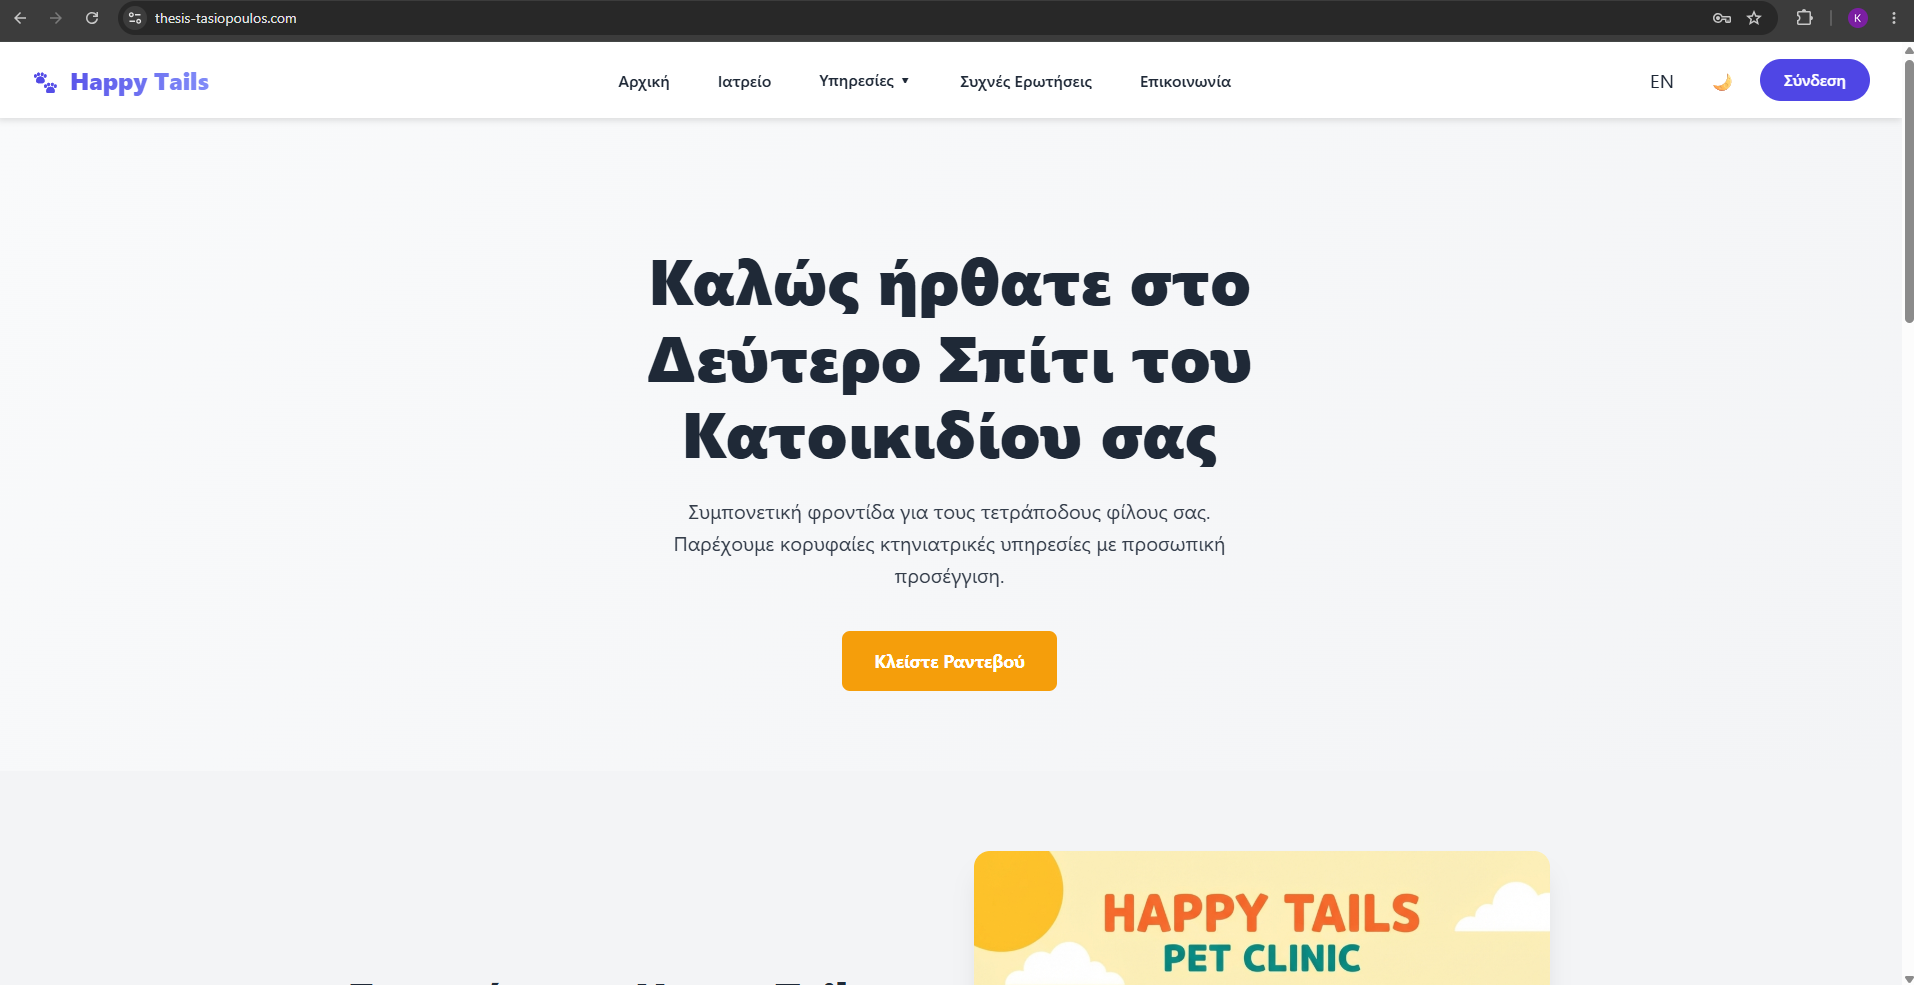
\includegraphics[width=\linewidth]{figures/application/landing-desktop.png}\\
\small (α) Desktop προβολή
\end{minipage}\hfill
\begin{minipage}[t]{0.24\textwidth}\centering
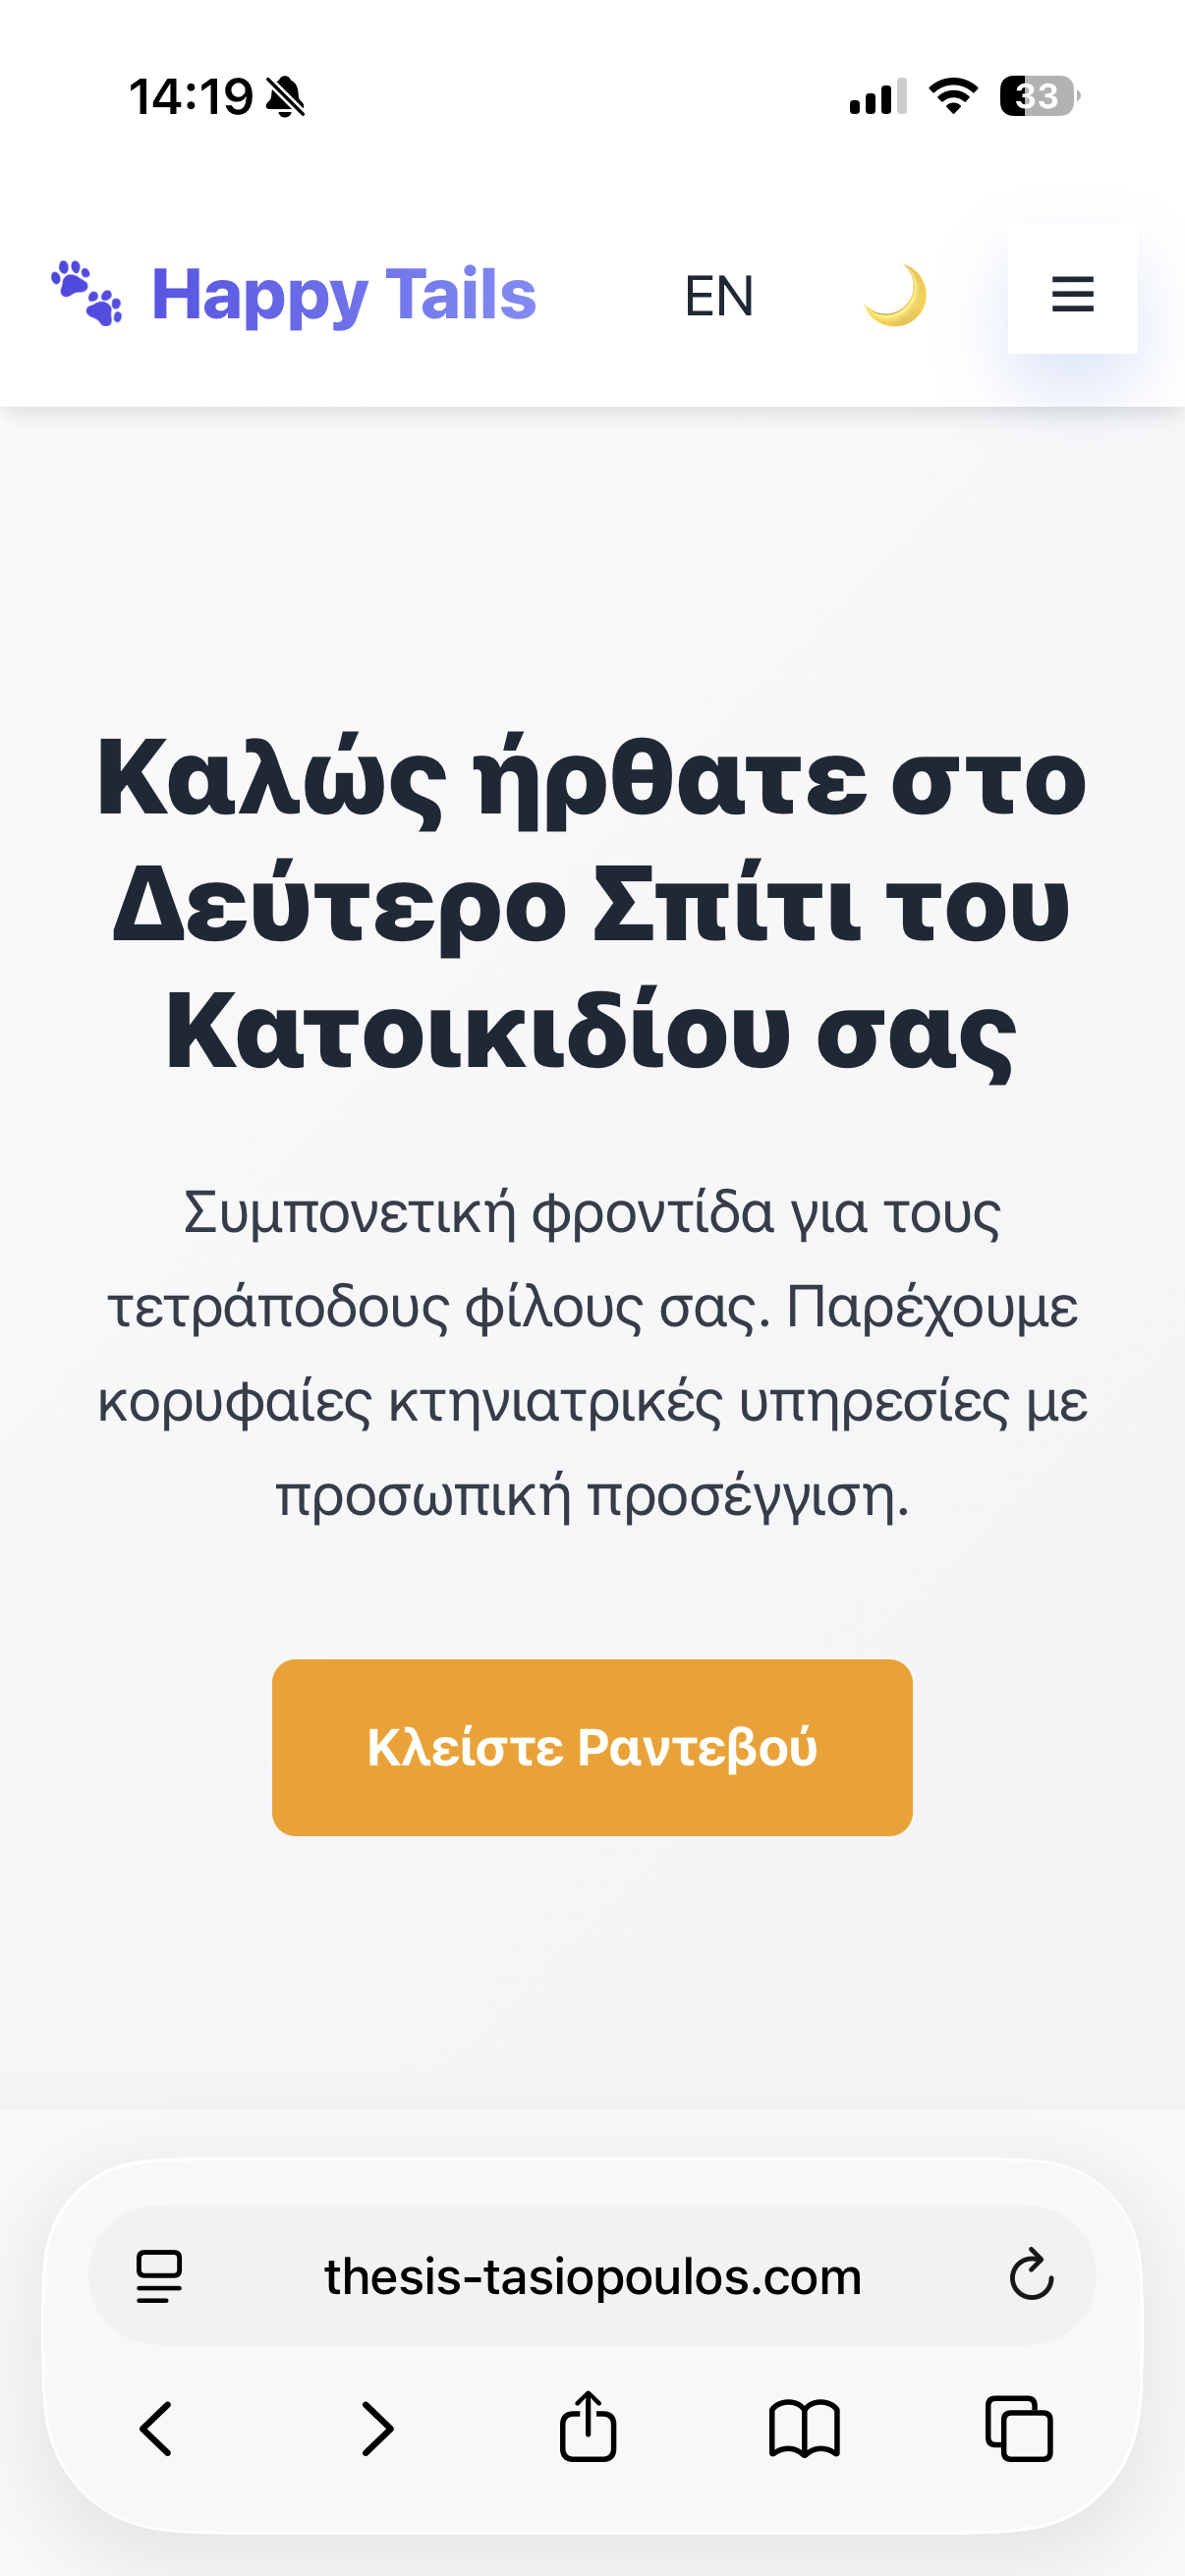
\includegraphics[width=\linewidth]{figures/application/landing-mobile.png}\\
\small (β) Mobile προβολή
\end{minipage}
\end{figure}

Η δημόσια αρχική σελίδα παρουσιάζει τον σκοπό της εφαρμογής και οδηγεί στη
σύνδεση ή στη φόρμα επικοινωνίας. Η mobile εικόνα δείχνει ότι η κεφαλίδα
συμπτύσσεται σε menu, ενώ η βασική ενέργεια παραμένει άμεσα διαθέσιμη. Στην
ενότητα της διπλωματικής παρουσιάζονται τα στοιχεία του έργου και
ενσωματωμένος χάρτης της πανεπιστημιακής τοποθεσίας. Ο χάρτης υλοποιείται με
responsive iframe και Google Maps place query, χωρίς application API key. Η
λύση είναι απλή για δημόσια πληροφορία τοποθεσίας, αλλά εξαρτά την απεικόνιση
από εξωτερικό πάροχο.

\begin{figure}[htbp]
\caption{Δημόσια ενότητα στοιχείων της διπλωματικής και ενσωματωμένος χάρτης
της πανεπιστημιακής τοποθεσίας.}
\label{fig:public-thesis-map}
\centering
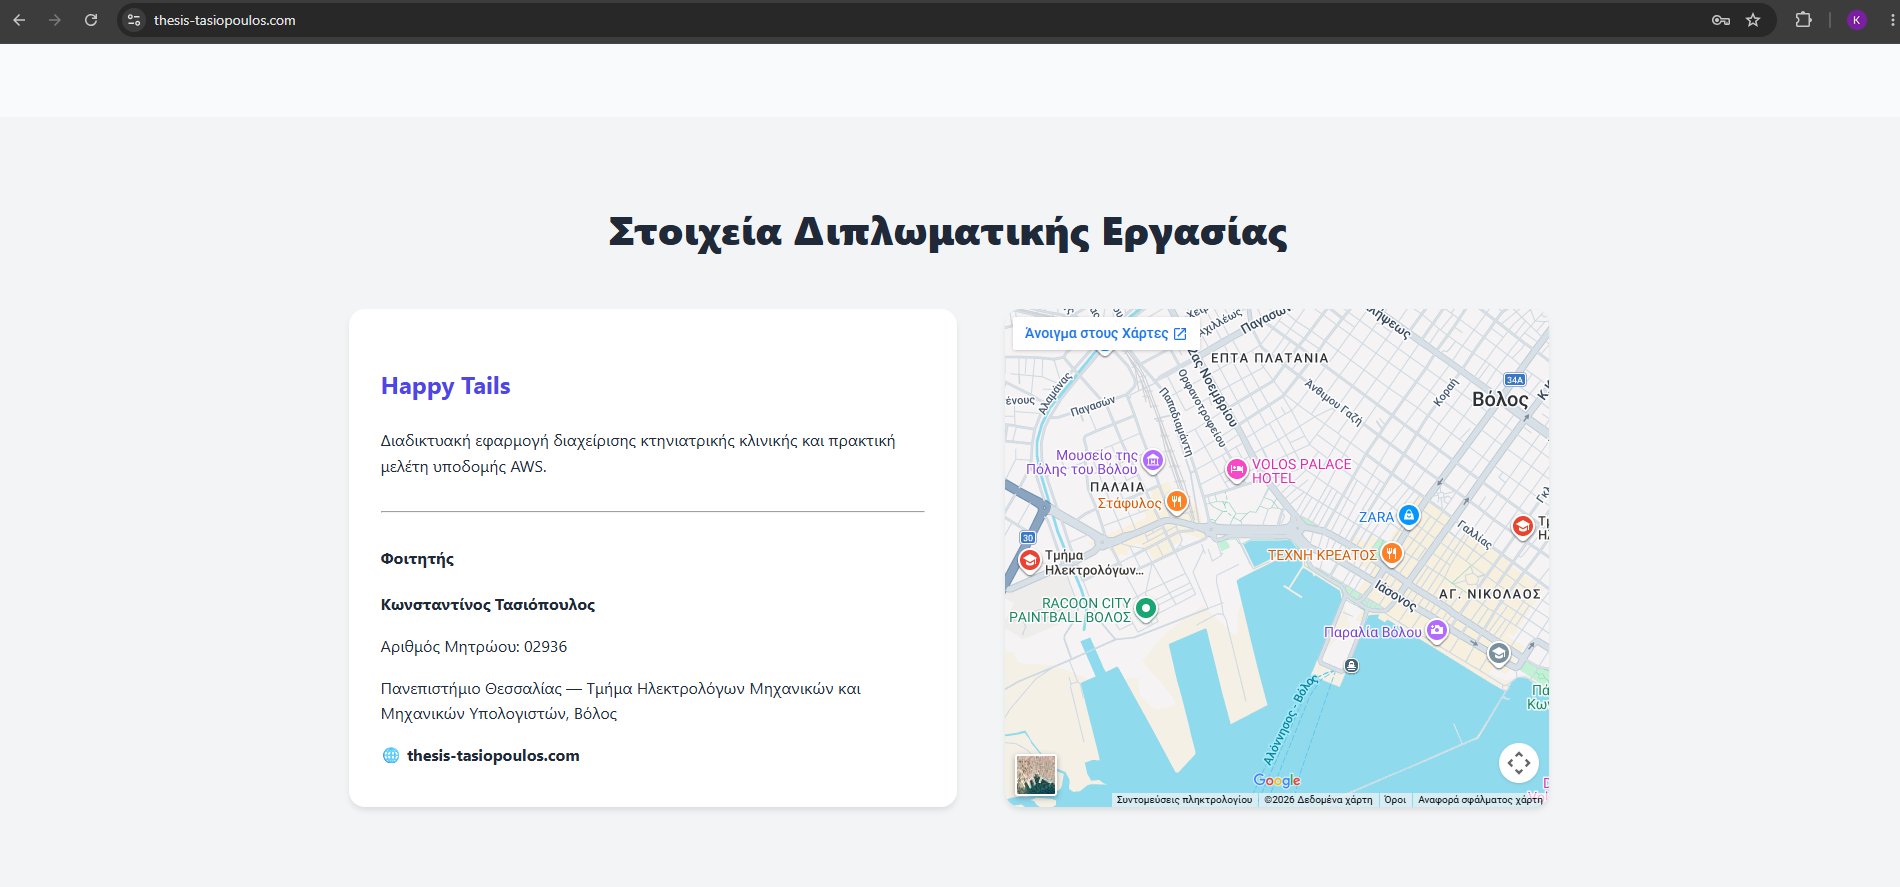
\includegraphics[width=0.9\textwidth]{figures/application/thesis-map-desktop.png}
\end{figure}

Μετά τη σύνδεση, ο πίνακας ελέγχου λειτουργεί ως σημείο προσανατολισμού. Στο
παράδειγμα εμφανίζεται ένα προσεχές ραντεβού για τη Λούνα και συνολικό πλήθος
ενός ραντεβού στην εβδομάδα. Τα δεδομένα δεν είναι στατικά στοιχεία της
σελίδας: προέρχονται από το \texttt{/api/dashboard} και υπολογίζονται από τις
αποθηκευμένες εγγραφές. Η mobile προβολή κρατά πρώτα τη σύνοψη και παρέχει
μόνιμη κάτω πλοήγηση, χρήσιμη όταν ο χρήστης χειρίζεται την εφαρμογή με το
ένα χέρι.

\begin{figure}[htbp]
\caption{Επιχειρησιακός πίνακας ελέγχου με πραγματική εγγραφή ραντεβού και
η αντίστοιχη responsive διάταξη.}
\label{fig:dashboard-responsive}
\centering
\begin{minipage}[t]{0.67\textwidth}\centering
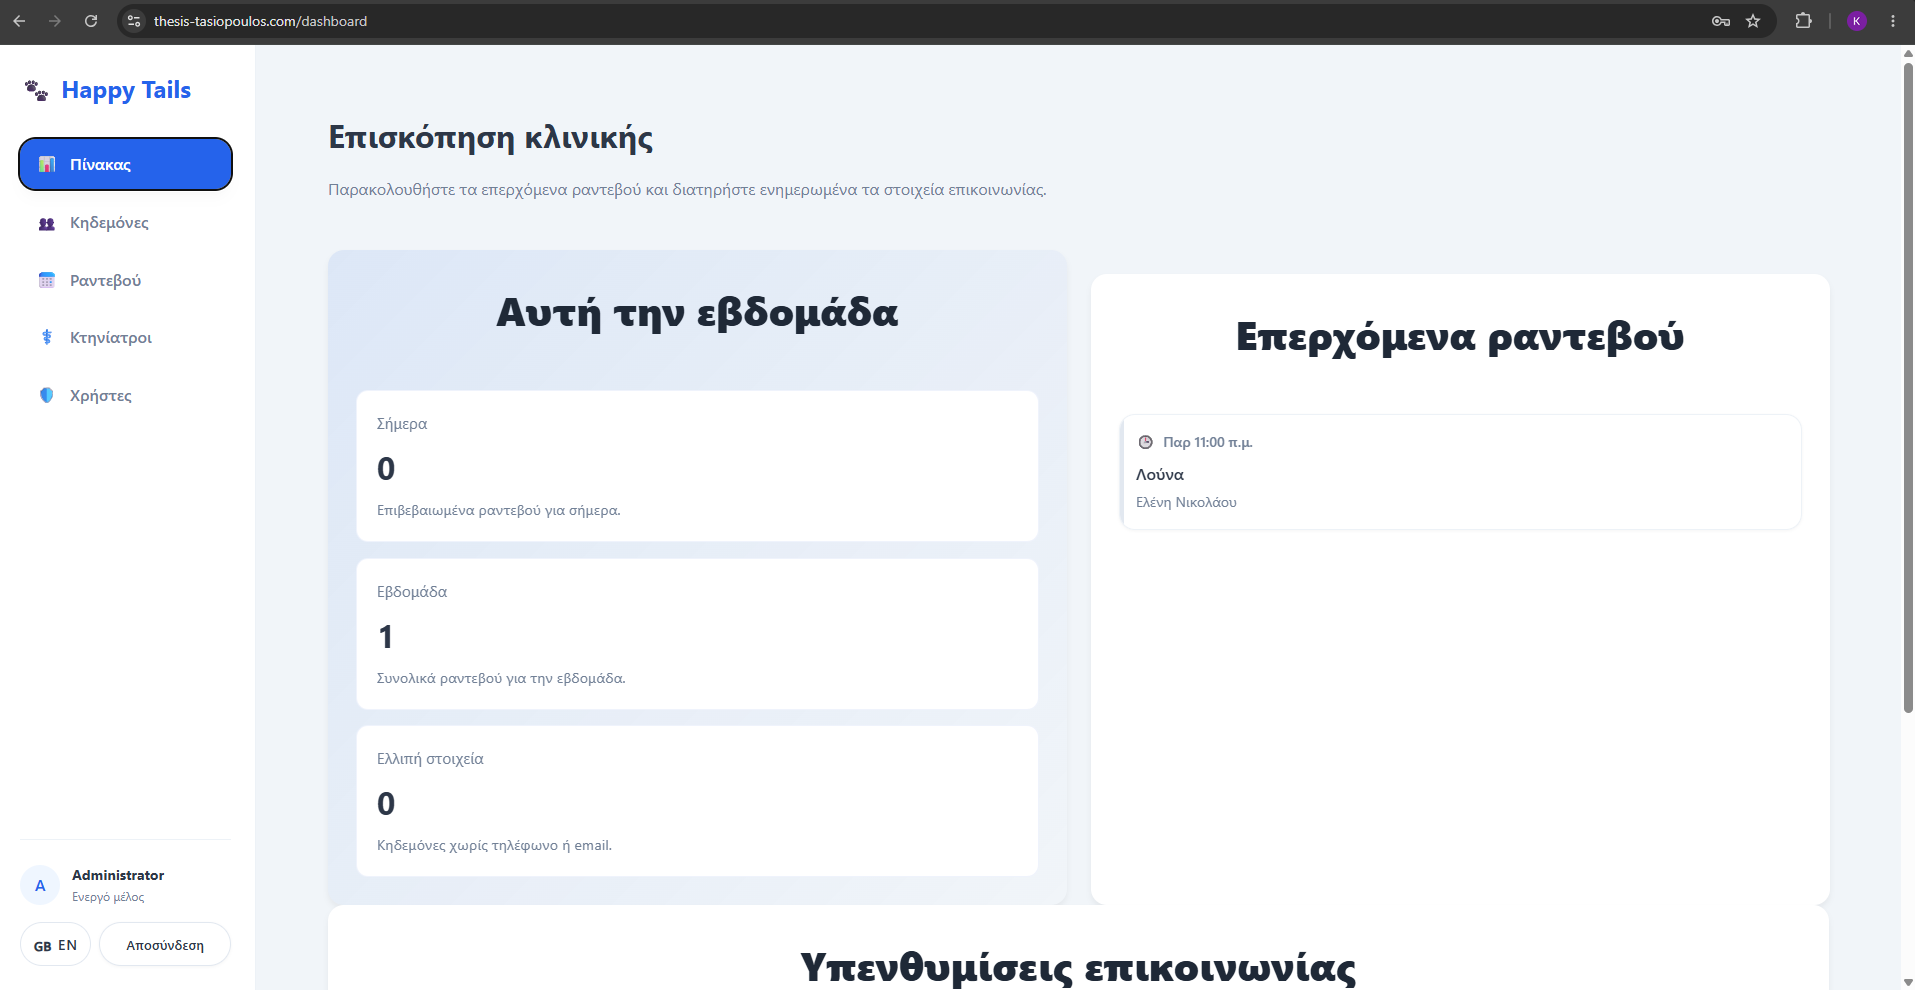
\includegraphics[width=\linewidth]{figures/application/dashboard-desktop.png}\\
\small (α) Σύνοψη σε desktop
\end{minipage}\hfill
\begin{minipage}[t]{0.24\textwidth}\centering
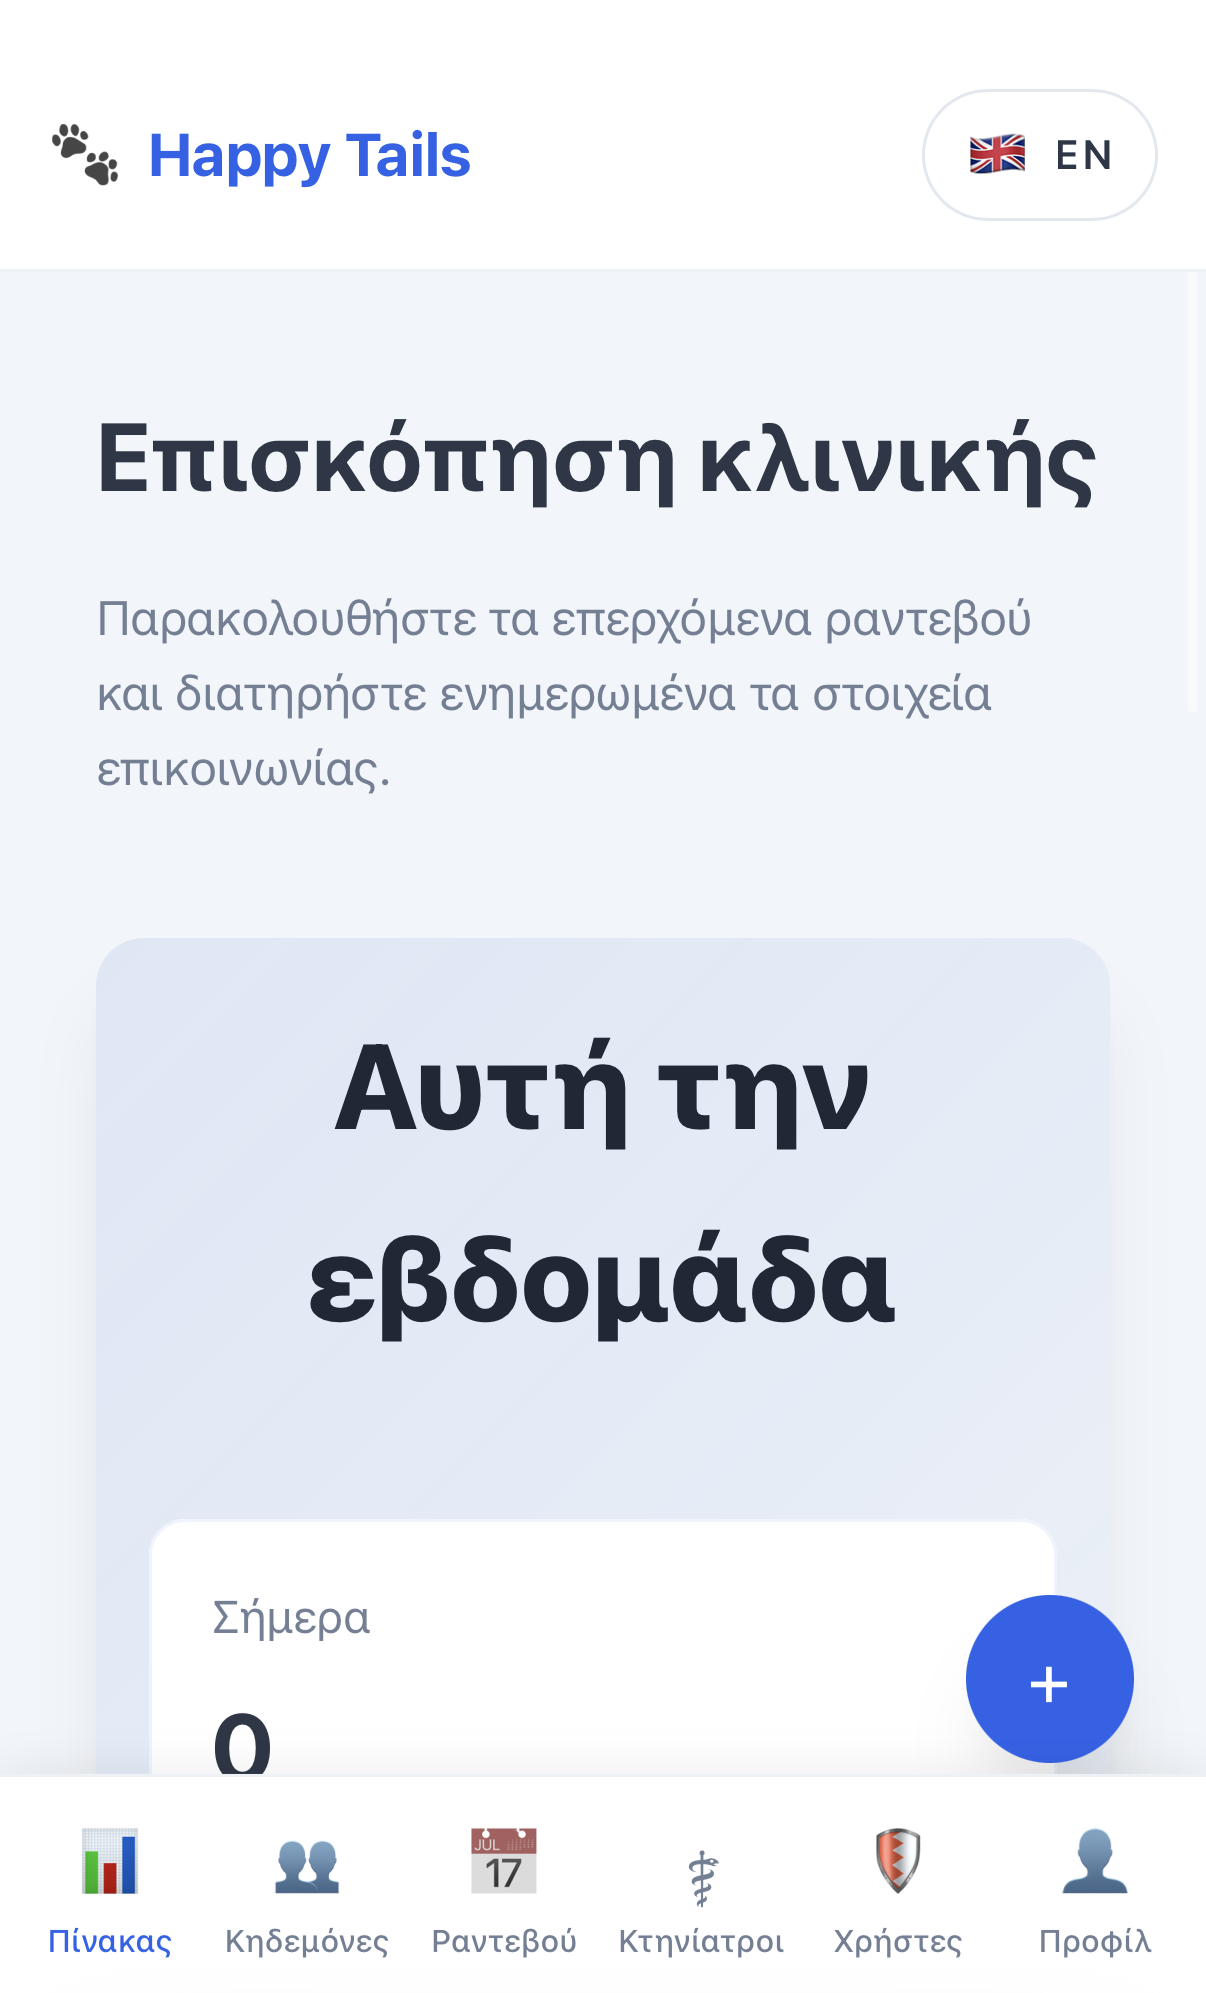
\includegraphics[width=\linewidth]{figures/application/dashboard-mobile.png}\\
\small (β) Σύνοψη σε κινητό
\end{minipage}
\end{figure}

\subsection{Καταχώριση ιδιοκτήτη και κατοικίδιου}

Η δημιουργία ιδιοκτήτη προηγείται της δημιουργίας κατοικίδιου, επειδή η
σχέση ιδιοκτησίας αποτελεί υποχρεωτικό μέρος του μοντέλου. Η φόρμα
ιδιοκτήτη αποστέλλει JSON στο \texttt{POST /api/owners}. Μετά την επιτυχή
απάντηση, ο χρήστης μεταφέρεται στην αναλυτική σελίδα και μπορεί να προσθέσει
το κατοικίδιο με \texttt{POST }\path{/api/owners/\{ownerId\}/pets}. Το frontend
ανανεώνει το query του ιδιοκτήτη και η νέα κάρτα εμφανίζεται χωρίς πλήρη
επαναφόρτωση της σελίδας.

Η Εικόνα~\ref{fig:owner-pet-responsive} παρουσιάζει το αποτέλεσμα της ροής.
Τα στοιχεία επικοινωνίας βρίσκονται μία φορά στο επίπεδο του ιδιοκτήτη, ενώ
οι γρήγορες ενέργειες του ζώου οδηγούν σε επίσκεψη, βάρος, εμβόλιο ή
απεικόνιση. Στο κινητό τα κουμπιά αναδιπλώνονται σε πλέγμα και η κάρτα
παραμένει ευανάγνωστη και οι βασικές ενέργειες είναι άμεσα διαθέσιμες χωρίς
οριζόντια μετατόπιση του κύριου περιεχομένου.

\begin{figure}[htbp]
\caption{Ολοκληρωμένη εγγραφή ιδιοκτήτη και κατοικίδιου σε desktop και
κινητό, με τις διαθέσιμες κλινικές ενέργειες.}
\label{fig:owner-pet-responsive}
\centering
\begin{minipage}[t]{0.67\textwidth}\centering
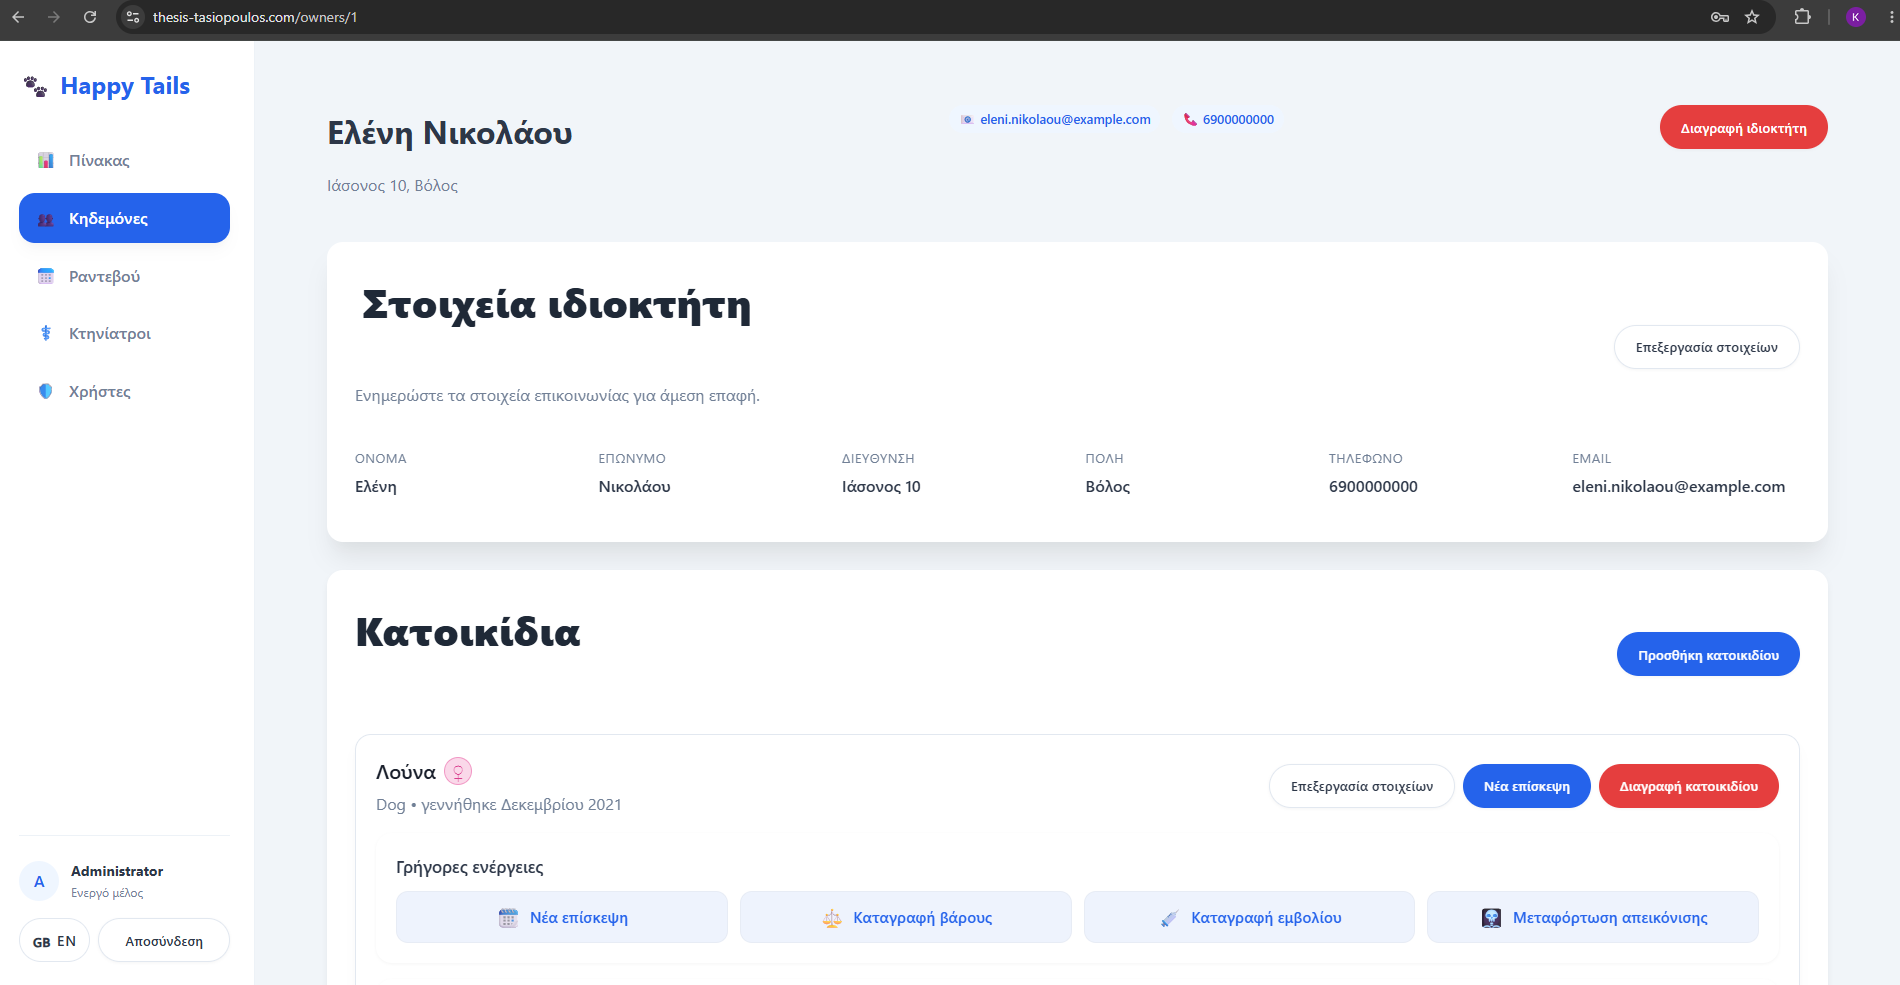
\includegraphics[width=\linewidth]{figures/application/owner-pet-desktop.png}\\
\small (α) Αναλυτική σελίδα ιδιοκτήτη
\end{minipage}\hfill
\begin{minipage}[t]{0.24\textwidth}\centering
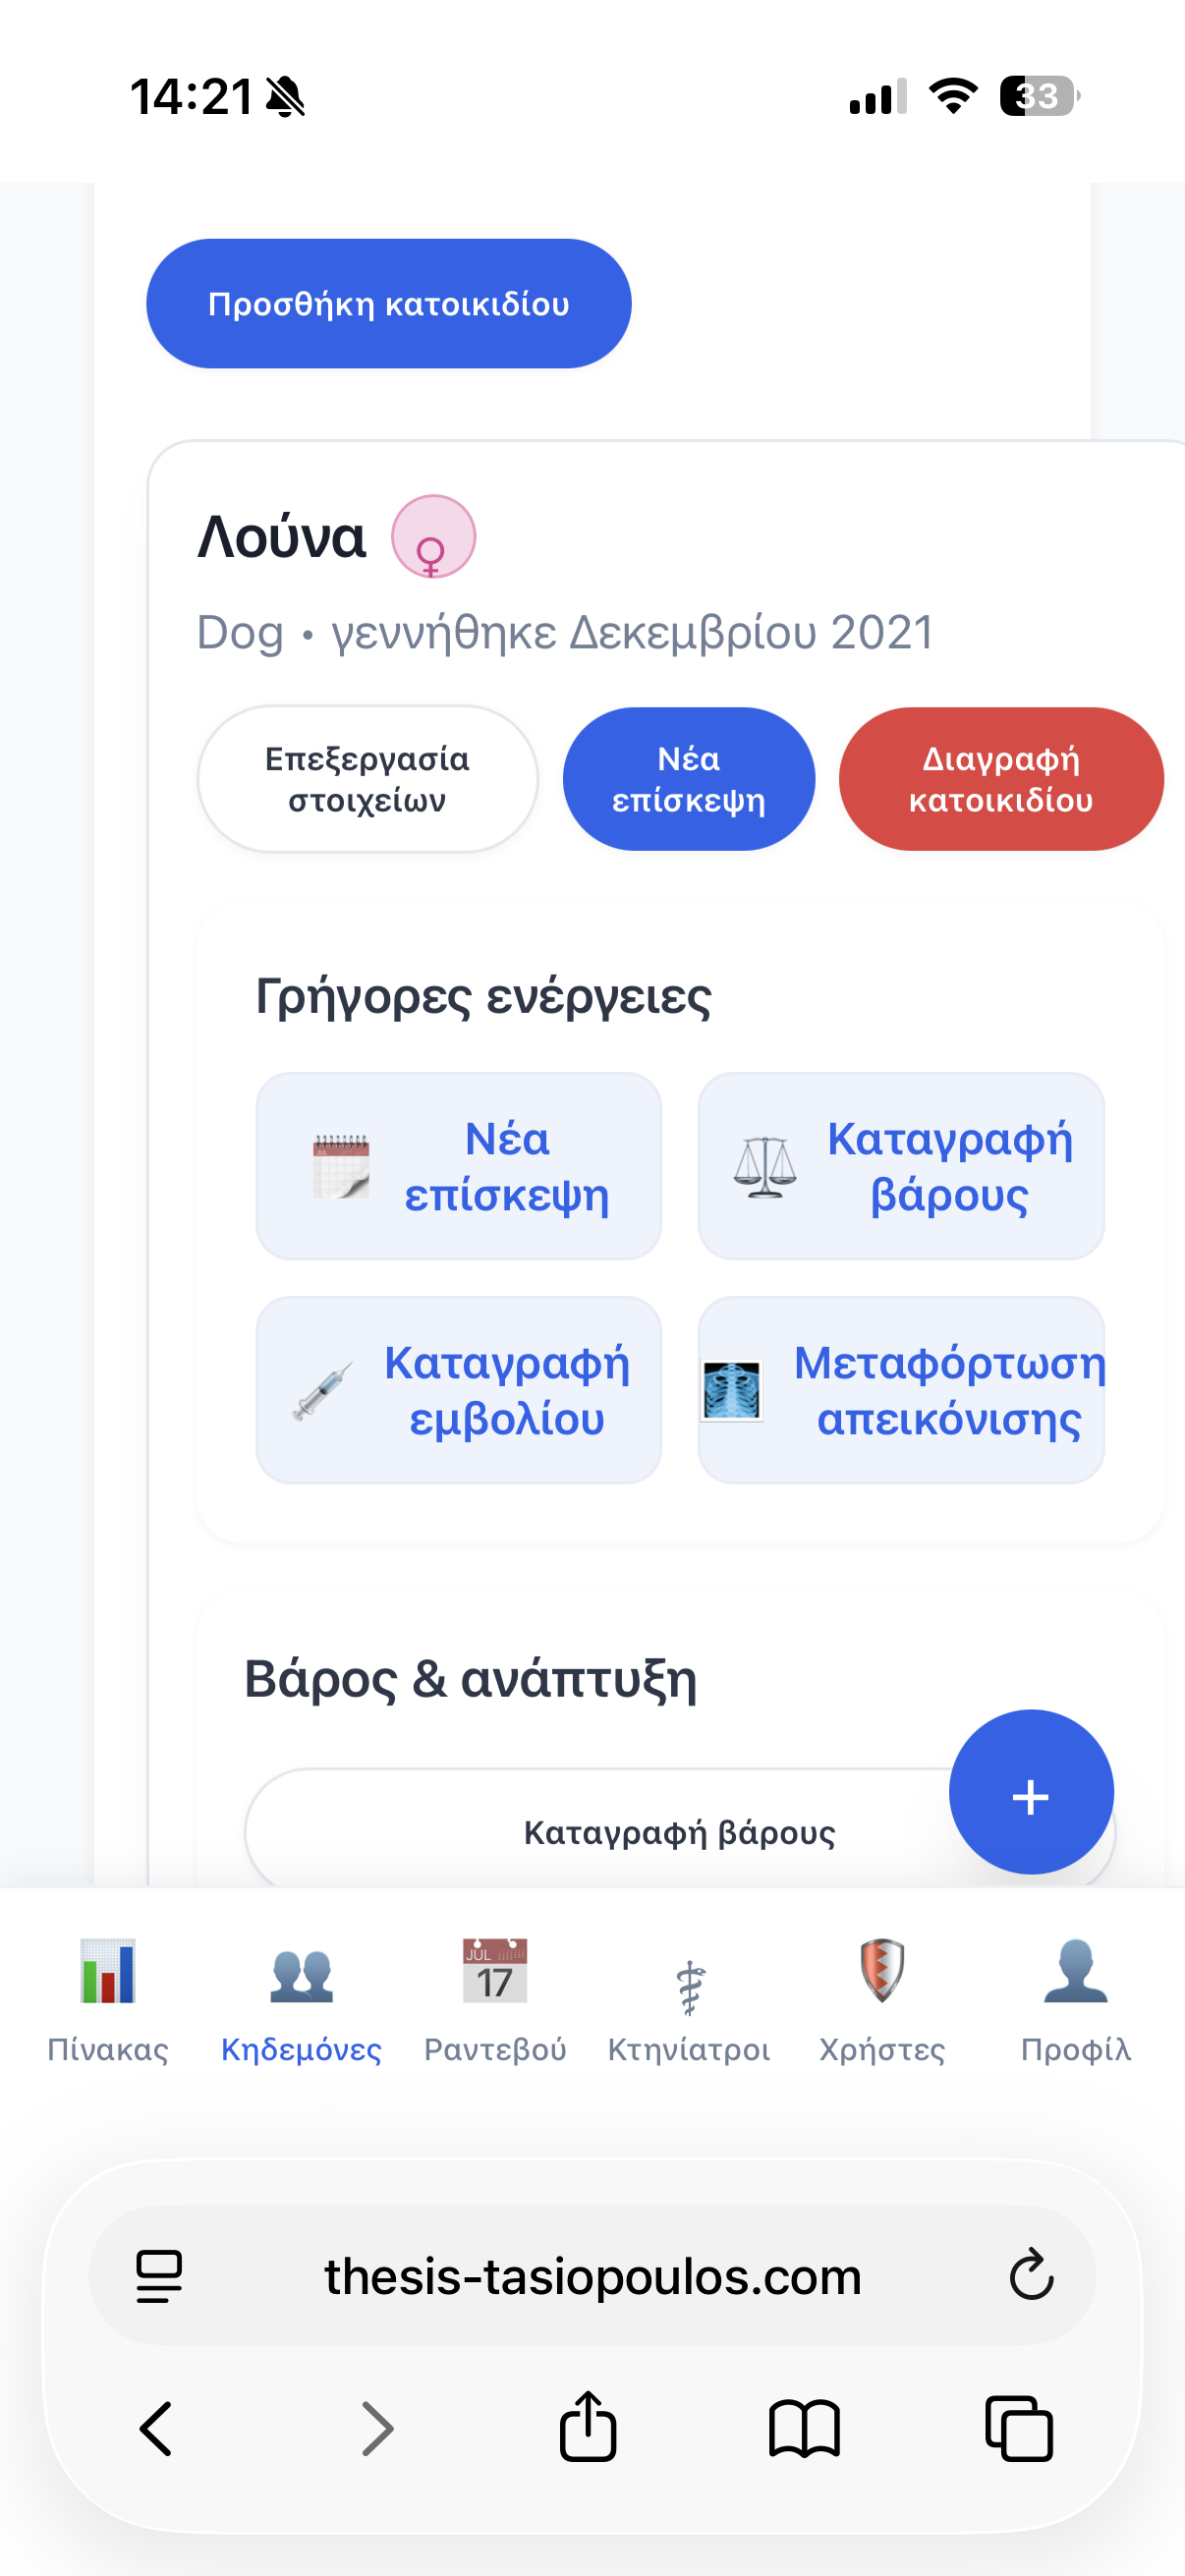
\includegraphics[width=\linewidth]{figures/application/owner-pet-mobile.png}\\
\small (β) Προσαρμογή των ενεργειών σε κινητό
\end{minipage}
\end{figure}

\subsection{Προγραμματισμός και διαχείριση ραντεβού}

Το εβδομαδιαίο ημερολόγιο συγκεντρώνει τα ραντεβού και επιτρέπει εναλλαγή
μήνα, εβδομάδας και ημέρας. Η επιλογή χρονικής θέσης ανοίγει φόρμα στην οποία
ορίζονται ιδιοκτήτης, κατοικίδιο, κτηνίατρος, ημερομηνία, ώρα και σημειώσεις.
Η επιλογή ιδιοκτήτη περιορίζει τα διαθέσιμα κατοικίδια, αποφεύγοντας
ασυνεπείς συνδυασμούς. Μετά το save, η επιτυχία εμφανίζεται μέσα στο drawer
και το calendar query ανανεώνεται.

Στη mobile προβολή οι ημέρες δεν συρρικνώνονται όλες στο πλάτος της οθόνης.
Η σύνοψη παραμένει σε οριζόντια λωρίδα και τα πλήκτρα προηγούμενης και
επόμενης εβδομάδας μετακινούν τη χρονική περίοδο. Η συμπεριφορά είναι
σκόπιμη: προτιμάται η αναγνωσιμότητα μιας ημέρας από ένα πλήρες αλλά
δυσανάγνωστο πλέγμα επτά πολύ στενών στηλών.

\begin{figure}[htbp]
\caption{Εβδομαδιαίο πρόγραμμα και προσαρμογή της πλοήγησης ραντεβού σε
κινητή συσκευή.}
\label{fig:calendar-responsive}
\centering
\begin{minipage}[t]{0.67\textwidth}\centering
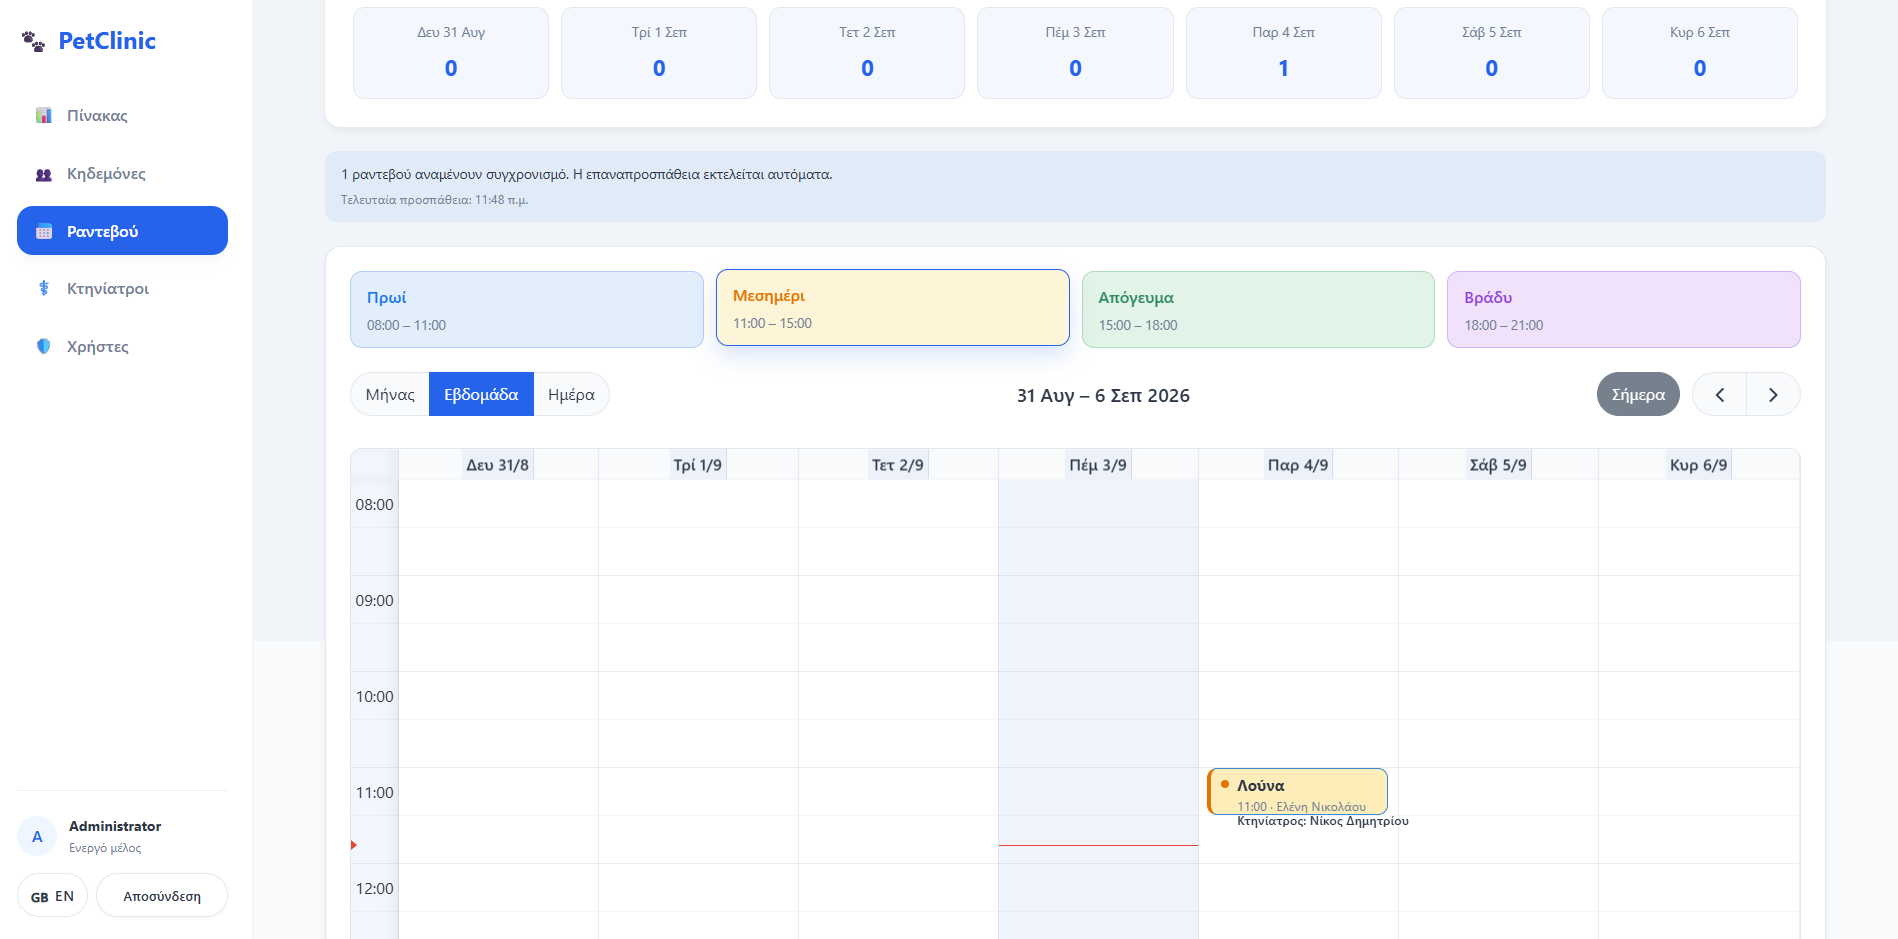
\includegraphics[width=\linewidth]{figures/application/calendar-week-desktop.png}\\
\small (α) Εβδομαδιαίο ημερολόγιο
\end{minipage}\hfill
\begin{minipage}[t]{0.24\textwidth}\centering
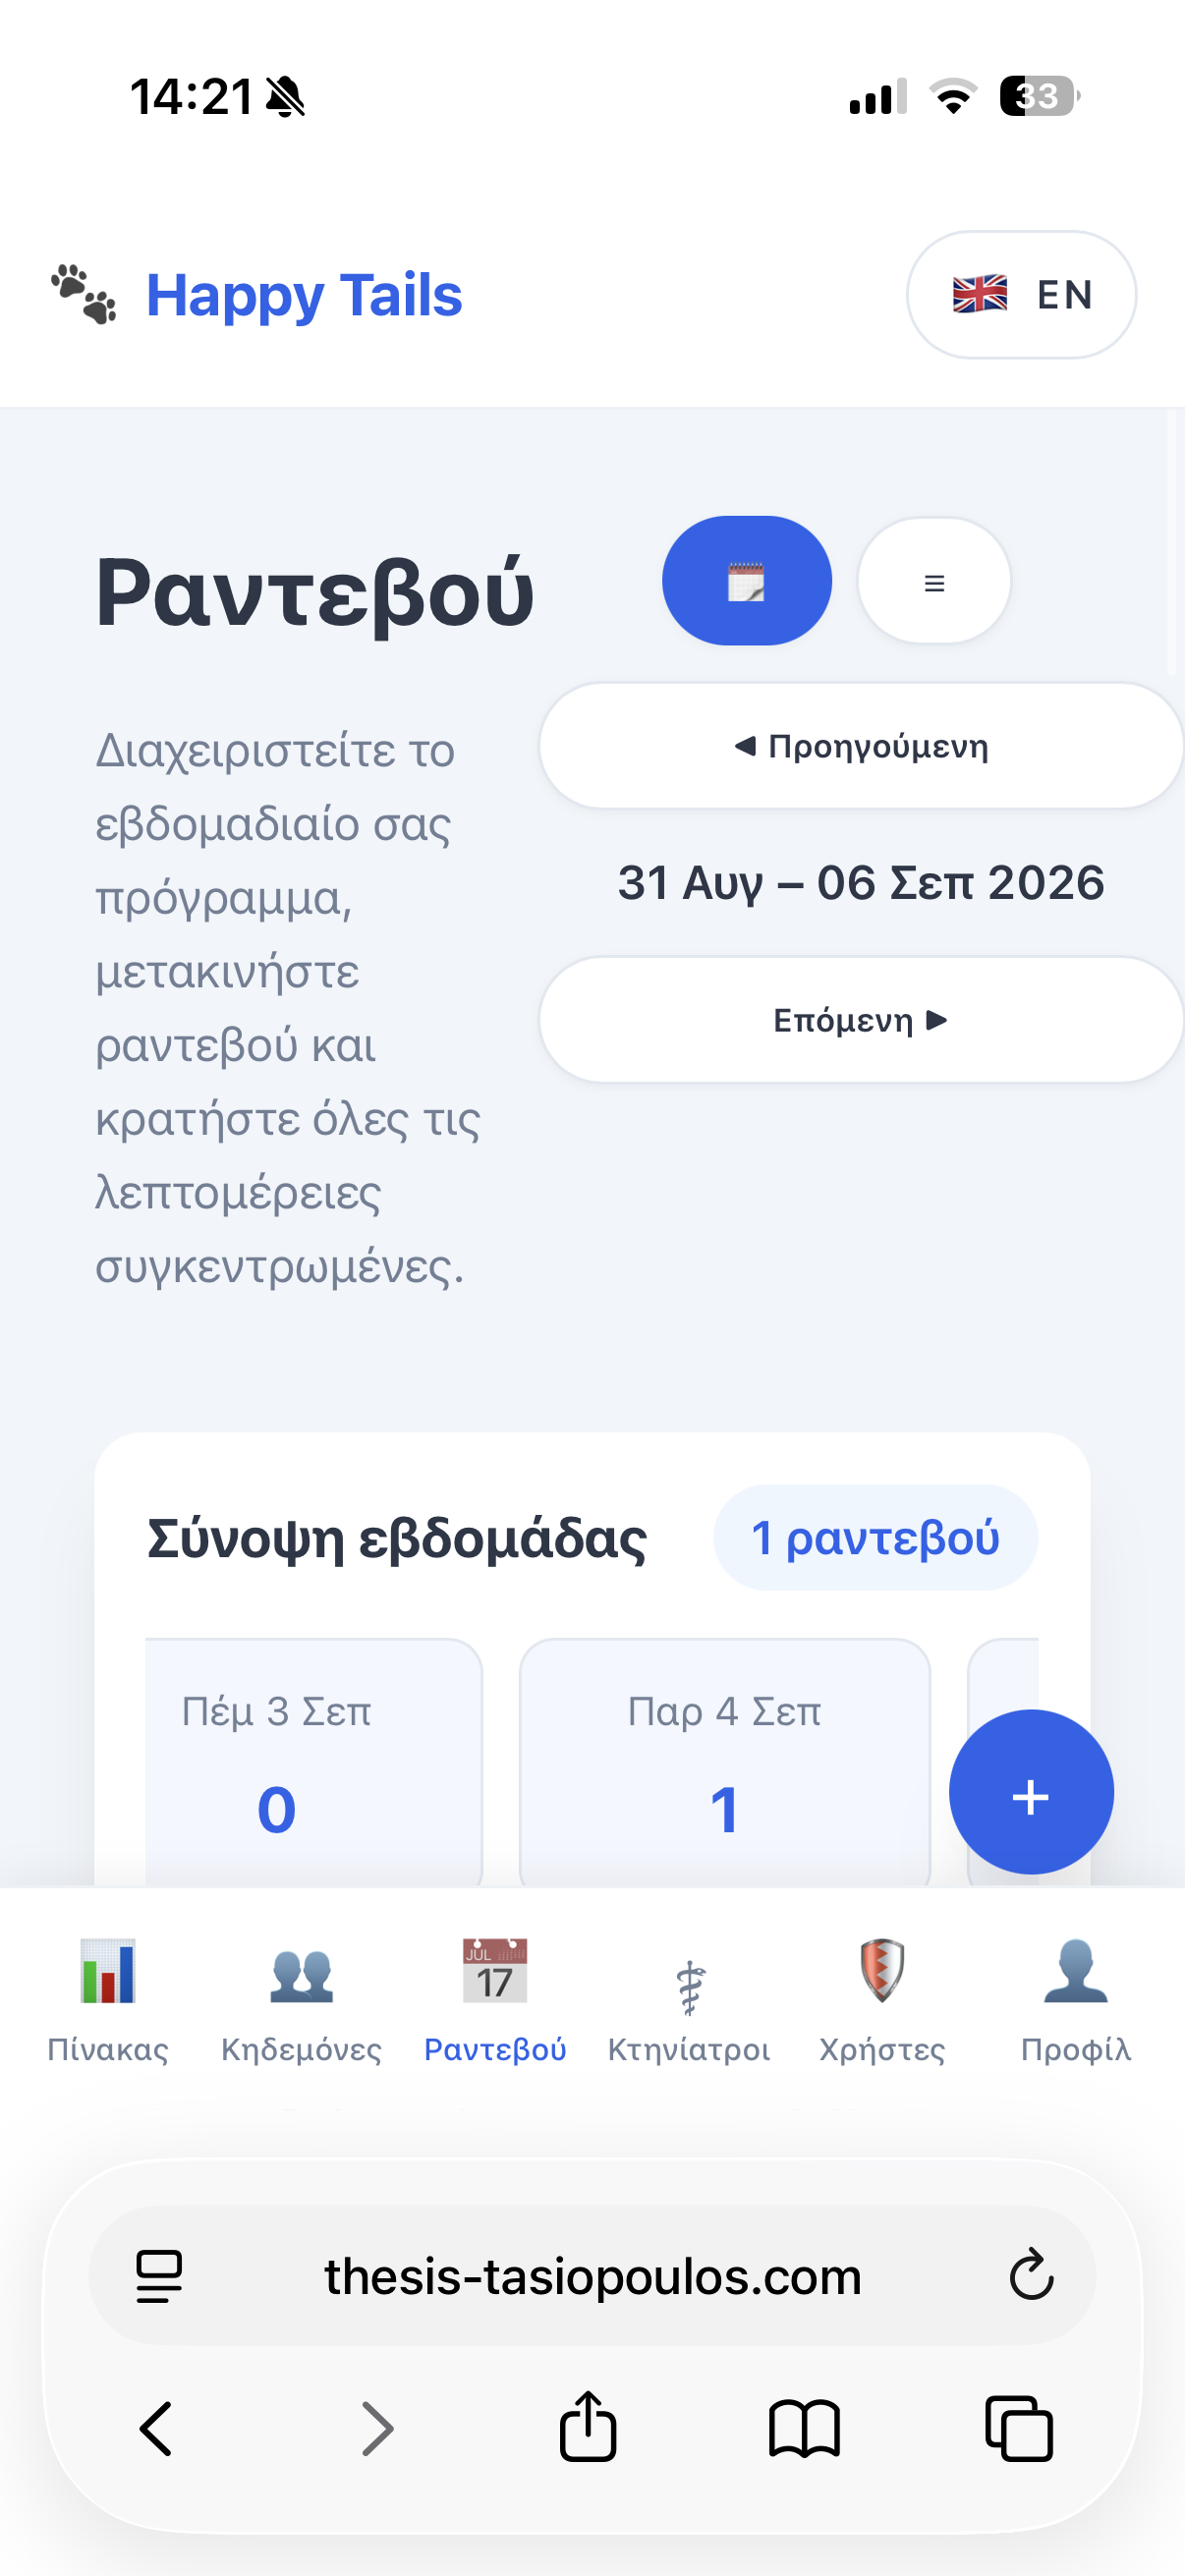
\includegraphics[width=\linewidth]{figures/application/appointments-mobile.png}\\
\small (β) Mobile σύνοψη και χρονική πλοήγηση
\end{minipage}
\end{figure}

\subsection{Διαχείριση επίσκεψης και κτηνιατρικού ιστορικού}

Η επιλογή ενός ραντεβού ανοίγει πλευρικό drawer χωρίς να χάνεται το πλαίσιο
του ημερολογίου. Ο χρήστης μπορεί να ενημερώσει τα στοιχεία της επίσκεψης
και να προσθέσει ιατρικό φάκελο. Η φόρμα φακέλου υποστηρίζει ζωτικές
μετρήσεις και αρχεία. Επειδή το περιεχόμενο είναι μεγαλύτερο από το ύψος
μιας συνηθισμένης οθόνης, το drawer διαθέτει ανεξάρτητη κατακόρυφη κύλιση και
σταθερή επικεφαλίδα. Το στιγμιότυπο μετά την αποθήκευση αποδεικνύει ότι η
μεταβολή ολοκληρώθηκε, ενώ η δεύτερη όψη δείχνει τις διαθέσιμες μετρήσεις και
την ήδη αποθηκευμένη εγγραφή.

\begin{figure}[htbp]
\caption{Αποθήκευση στοιχείων ραντεβού και καταχώριση ζωτικών μετρήσεων στον
ιατρικό φάκελο από το ίδιο πλευρικό drawer.}
\label{fig:appointment-record}
\centering
\begin{minipage}[t]{0.49\textwidth}\centering
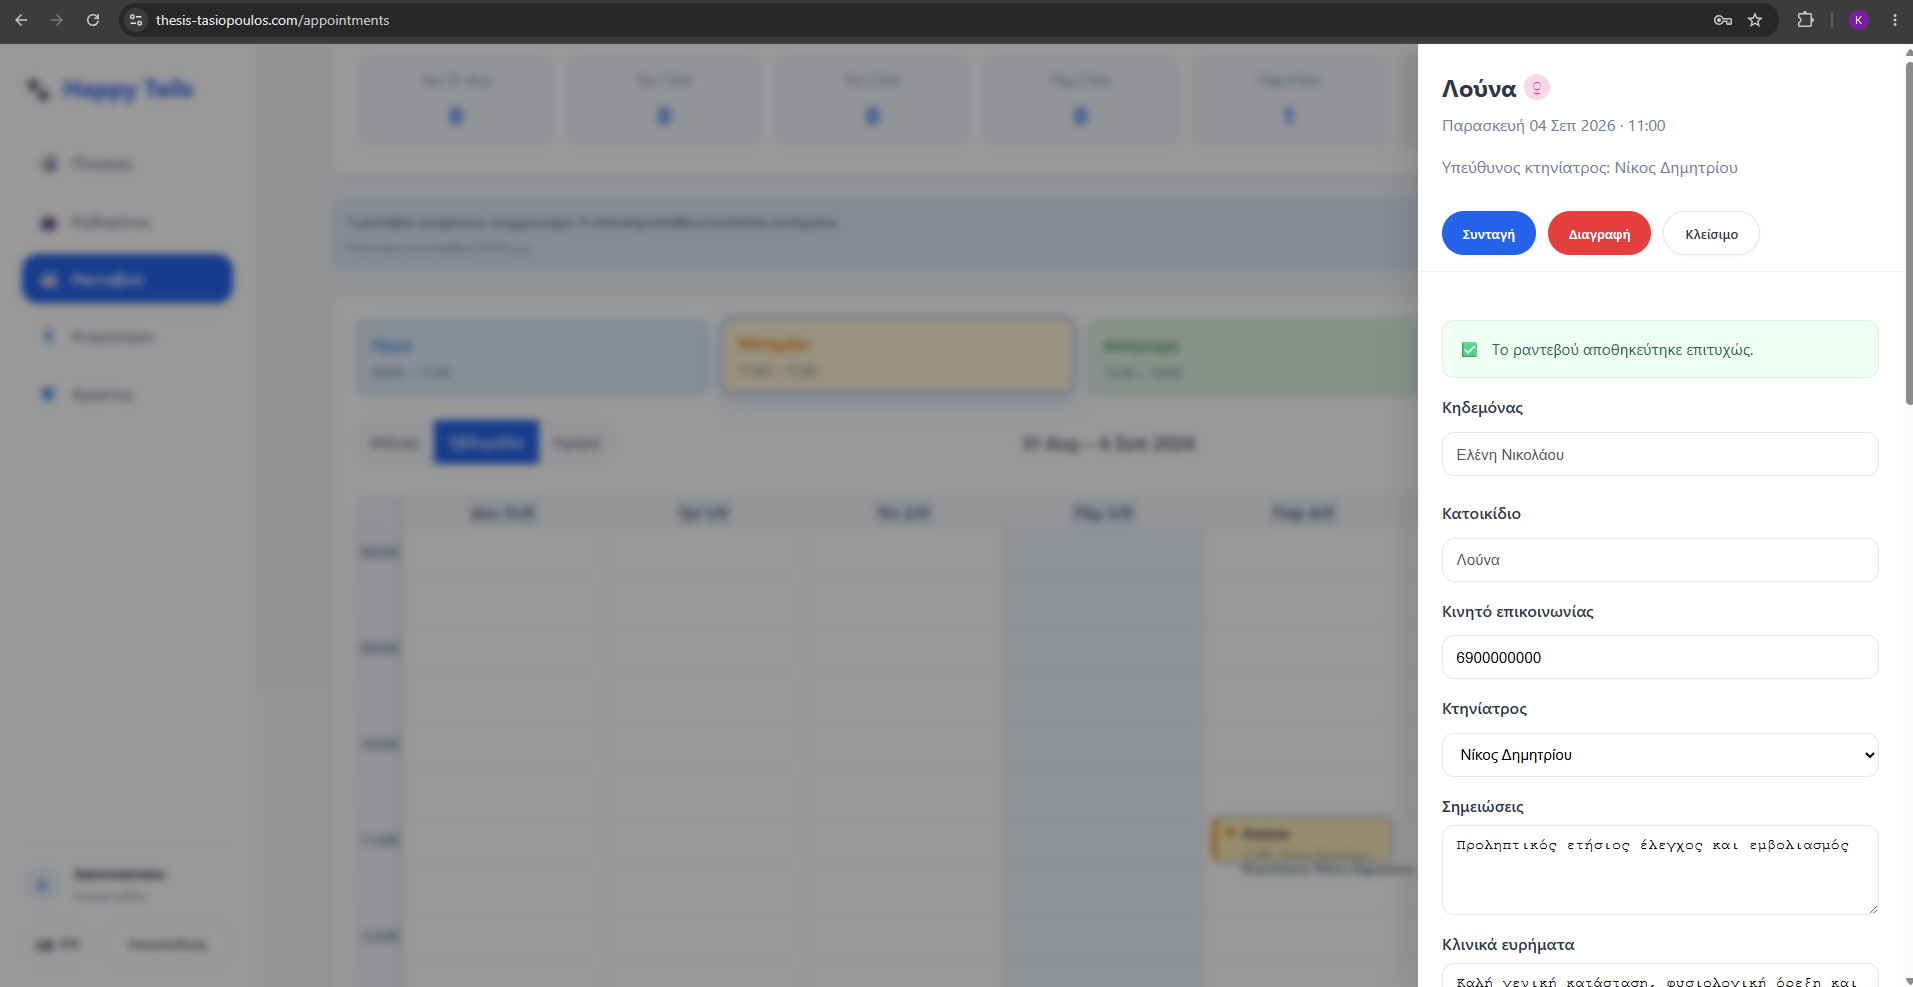
\includegraphics[width=\linewidth]{figures/application/appointment-save-desktop.png}\\
\small (α) Επιβεβαίωση επιτυχούς αποθήκευσης
\end{minipage}\hfill
\begin{minipage}[t]{0.49\textwidth}\centering
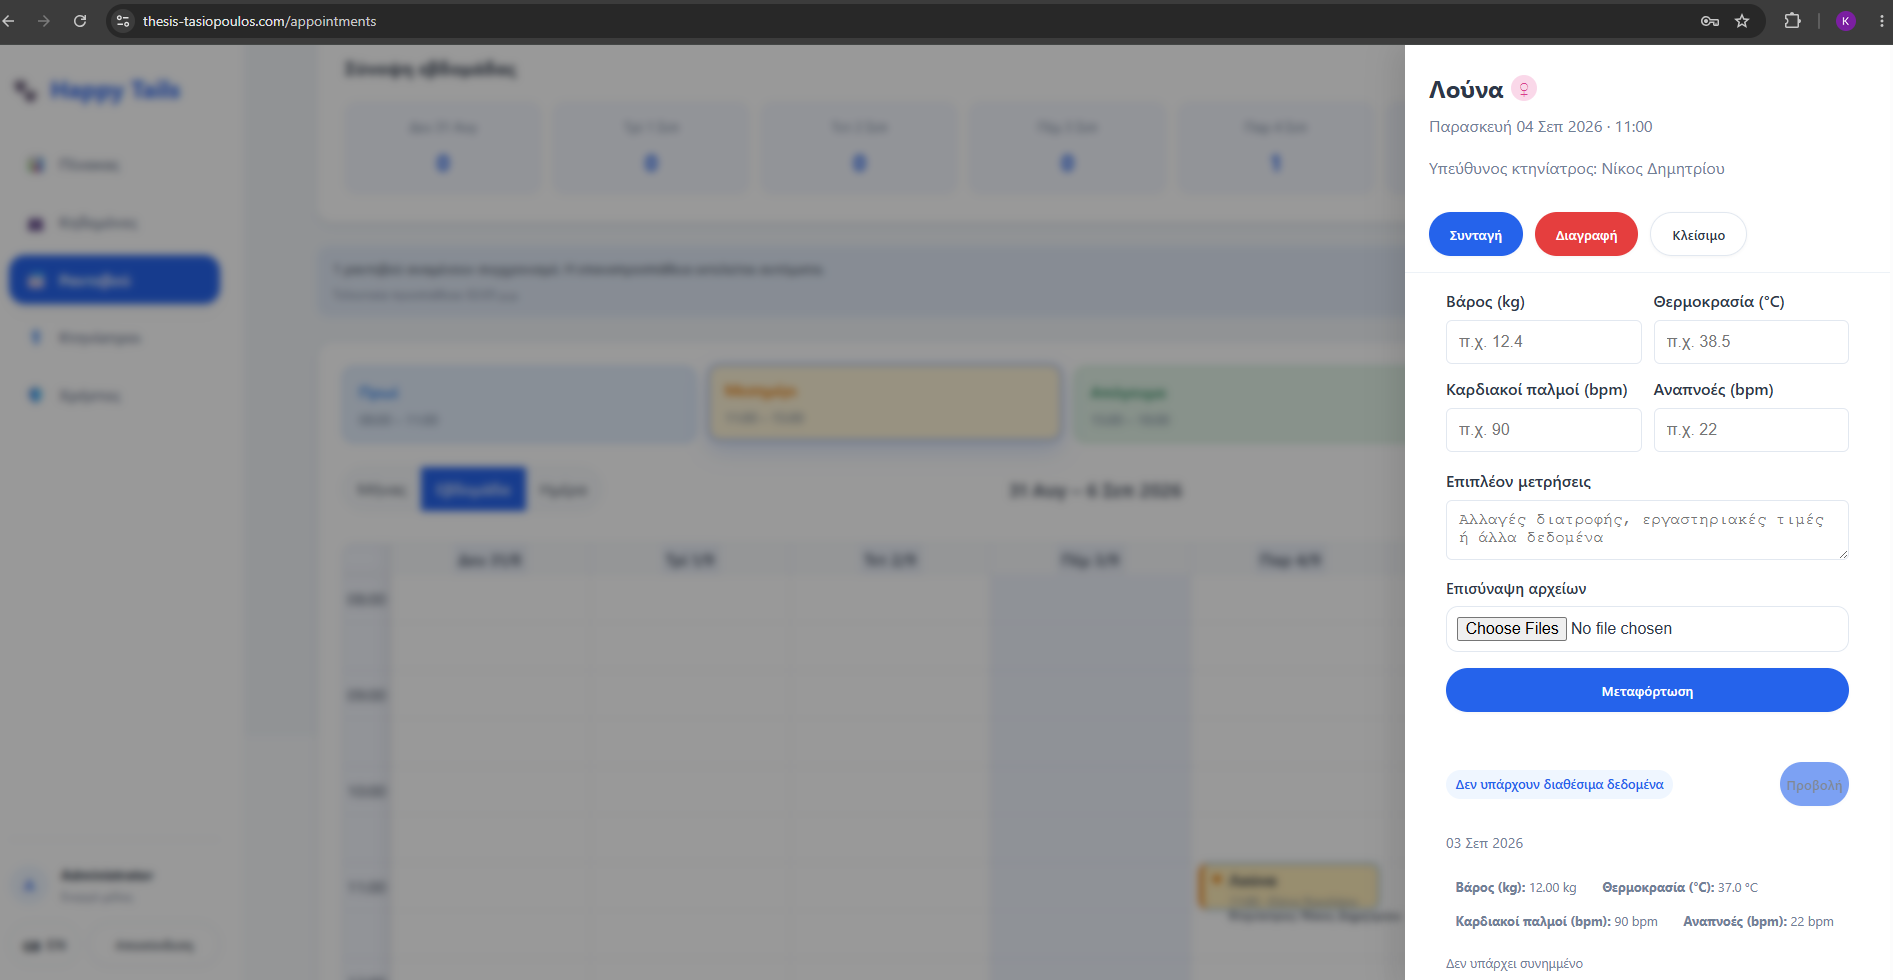
\includegraphics[width=\linewidth]{figures/application/health-record-desktop.png}\\
\small (β) Μετρήσεις και συνημμένα ιατρικού φακέλου
\end{minipage}
\end{figure}

Η καταχώριση βάρους τροφοδοτεί τη γραφική παράσταση στην καρτέλα του
κατοικίδιου. Το γράφημα δεν αποτελεί ξεχωριστή αποθήκη δεδομένων· είναι
παράγωγη απεικόνιση των health records που περιέχουν τιμή βάρους. Αντίστοιχα,
η συνταγή χρησιμοποιεί τα στοιχεία της κλινικής, του ζώου και του ιδιοκτήτη
για να δημιουργήσει εκτυπώσιμη προβολή, την οποία ο browser μπορεί να
αποθηκεύσει ως PDF. Με αυτόν τον τρόπο τα δεδομένα που καταχωρίστηκαν για την
κλινική εργασία μπορούν να εξαχθούν σε μορφή κατάλληλη για παράδοση.

\begin{figure}[htbp]
\caption{Παράγωγα της κλινικής πληροφορίας: διάγραμμα πορείας βάρους και
εκτυπώσιμη συνταγή.}
\label{fig:clinical-outputs}
\centering
\begin{minipage}[t]{0.49\textwidth}\centering
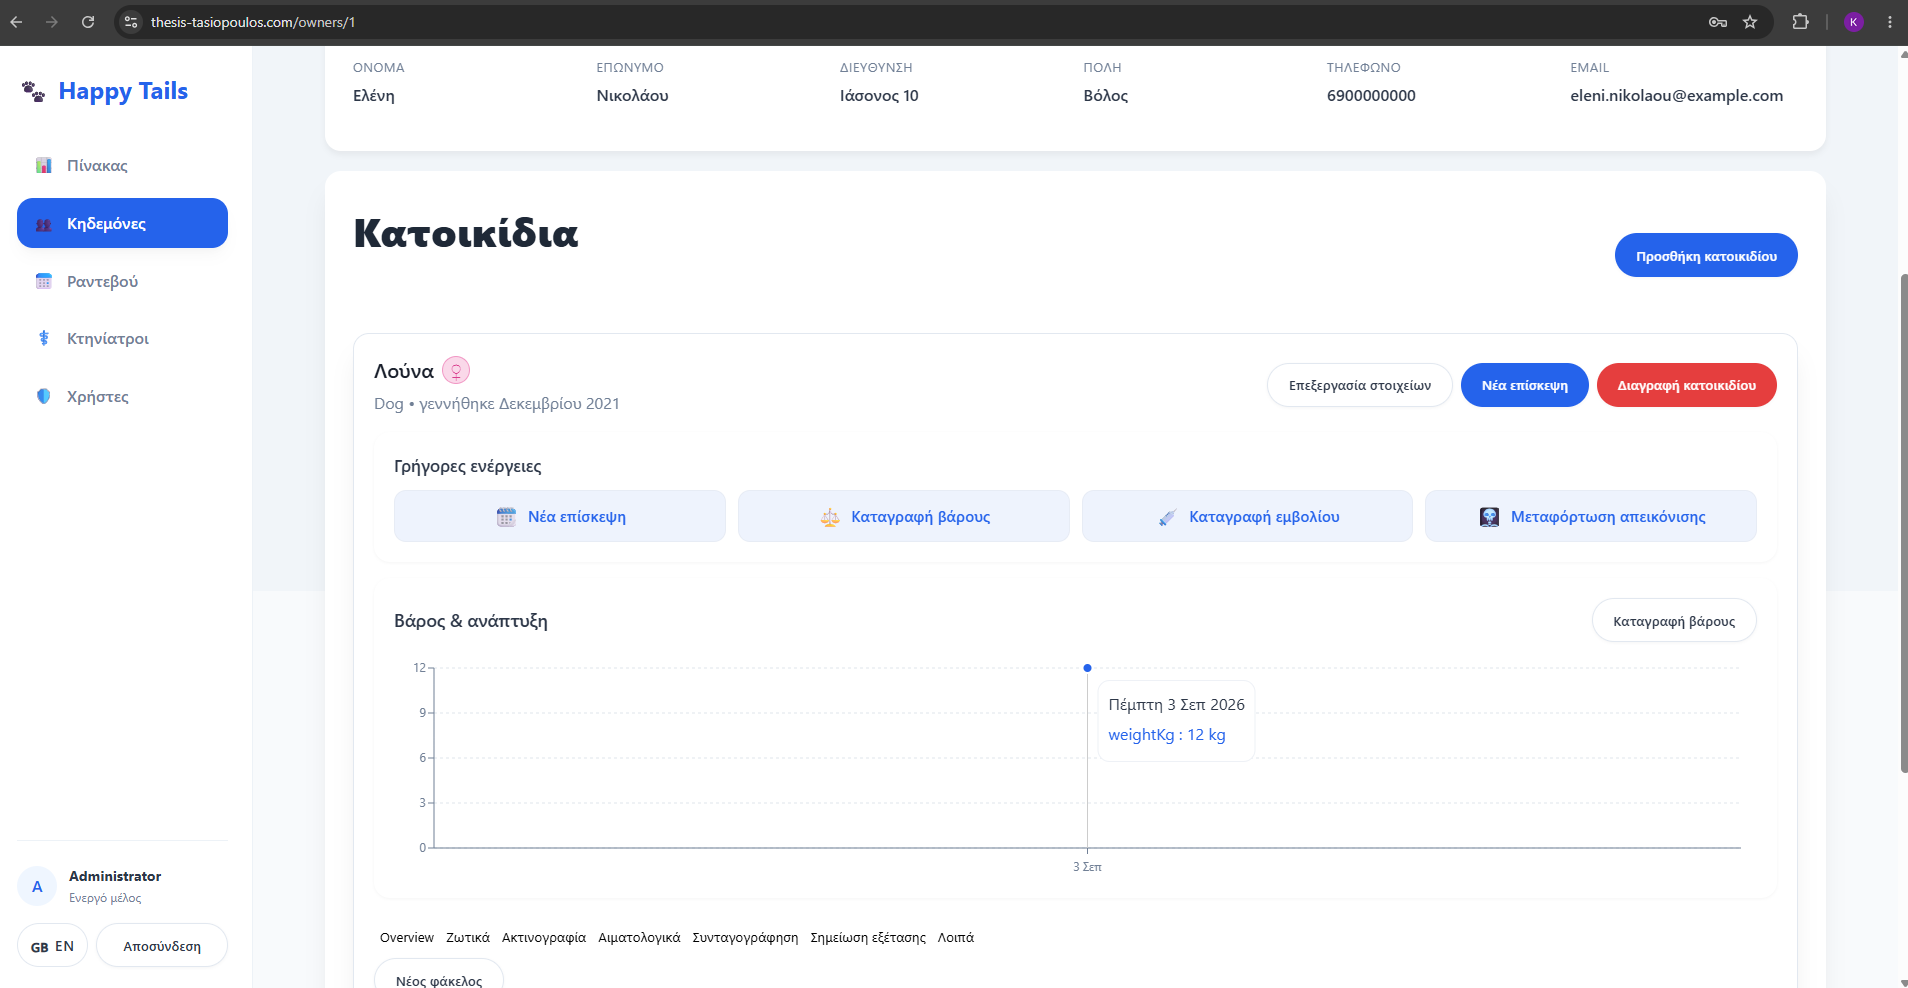
\includegraphics[width=\linewidth]{figures/application/weight-chart-desktop.png}\\
\small (α) Ιστορικό βάρους
\end{minipage}\hfill
\begin{minipage}[t]{0.49\textwidth}\centering
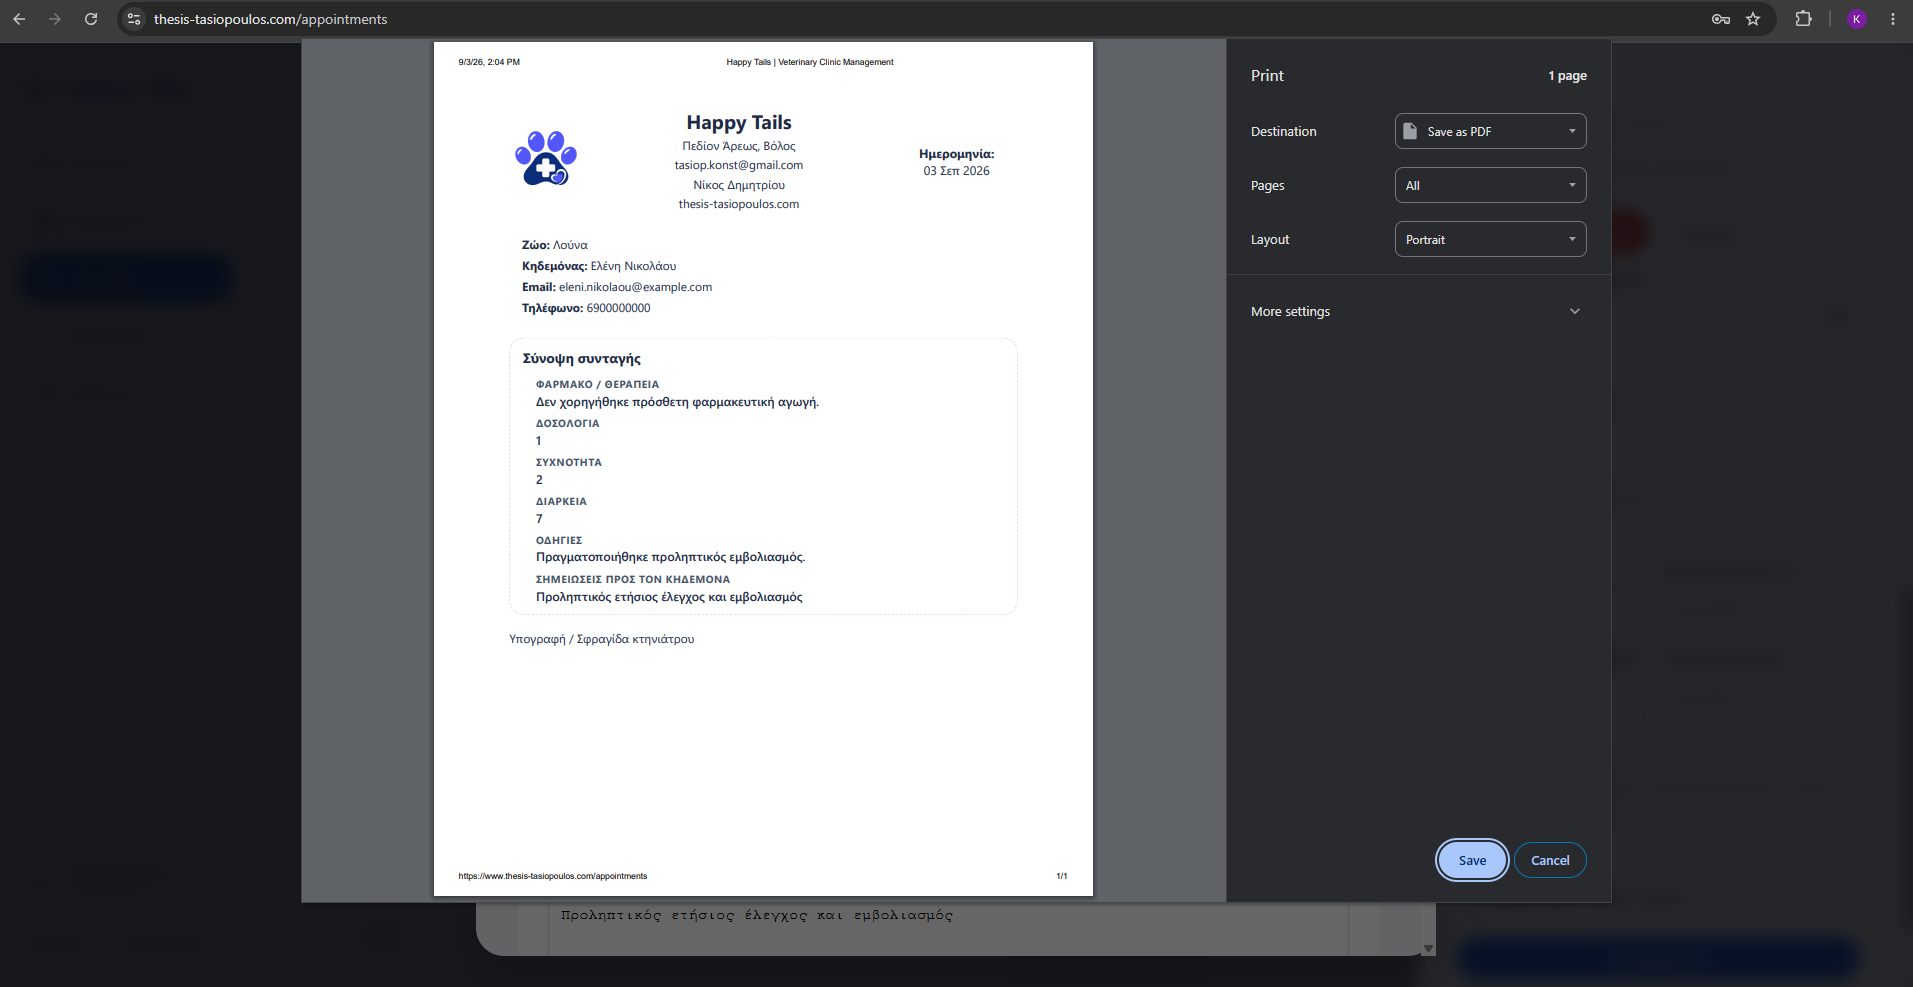
\includegraphics[width=\linewidth]{figures/application/prescription-print-desktop.png}\\
\small (β) Προεπισκόπηση εκτύπωσης συνταγής
\end{minipage}
\end{figure}

\subsection{Διοίκηση χρηστών}

Η σελίδα χρηστών διαχωρίζει εκκρεμείς, ενεργούς και αποκλεισμένους
λογαριασμούς. Από εδώ ο διαχειριστής μπορεί να εγκρίνει έναν χρήστη, να τον
απενεργοποιήσει, να τον αποκλείσει ή να ενημερώσει τους ρόλους του. Η
διεύθυνση email εμφανίζεται ώστε η απόφαση να συνδέεται με συγκεκριμένη
αίτηση. Στην Εικόνα~\ref{fig:admin-users} ο ενεργός λογαριασμός της
εγκατάστασης εμφανίζεται με τη διεύθυνση επικοινωνίας που έχει οριστεί στην
production παραμετροποίηση.

\begin{figure}[htbp]
\caption{Διοικητική προβολή ενεργών χρηστών και ενεργειών ελέγχου πρόσβασης.}
\label{fig:admin-users}
\centering
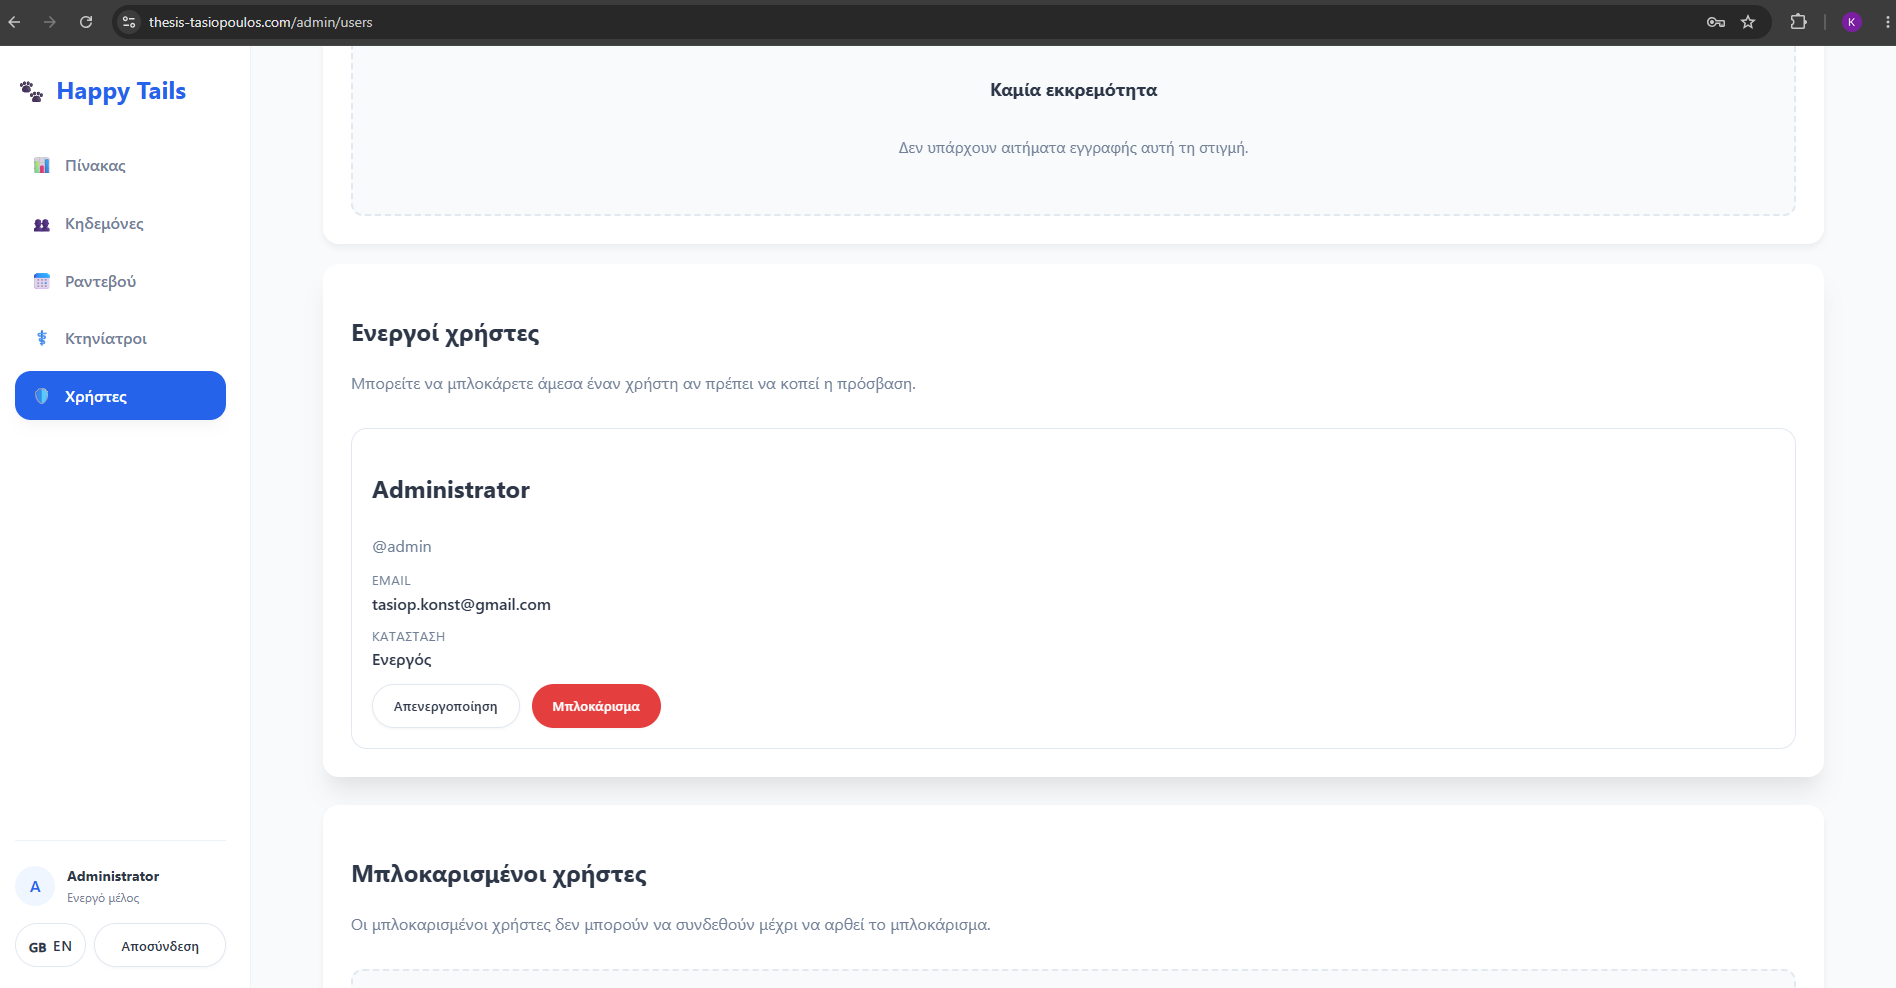
\includegraphics[width=0.9\textwidth]{figures/application/admin-users-desktop.png}
\end{figure}

\section{Εξωτερικές ενσωματώσεις και όρια λειτουργίας}

Η ενσωμάτωση Google Calendar αφορά τον συνδεδεμένο λογαριασμό του μέλους
προσωπικού, όχι το email του ιδιοκτήτη του ζώου. Ο χρήστης εξουσιοδοτεί ρητά
την εφαρμογή μέσω OAuth~2.0 \cite{rfc6749,google2026calendar} και το backend μπορεί κατόπιν να δημιουργεί,
ενημερώνει ή διαγράφει το αντίστοιχο calendar event. Τα δοκιμαστικά
\texttt{example.com} emails των ιδιοκτητών δεν εμποδίζουν αυτή τη ροή,
επειδή χρησιμοποιούνται ως στοιχεία επικοινωνίας και όχι ως λογαριασμοί
πρόσβασης στο ημερολόγιο. Στην παρούσα φάση ο κώδικας υπάρχει, αλλά η
production σύνδεση και η end-to-end δημιουργία event παραμένουν προς τελική
επαλήθευση.

Η υπηρεσία email είναι επίσης προαιρετική εξωτερική εξάρτηση. Η ροή
επιβεβαίωσης έχει υλοποιηθεί στο Spring Boot, όμως η χρήση Amazon SES
\cite{aws2026ses} θα
χαρακτηριστεί ενεργή μόνο μετά τη δημιουργία verified identity και την
επιτυχή παραλαβή μηνύματος από το production περιβάλλον. Η σαφής καταγραφή
αυτών των ορίων αποτρέπει τη σύγχυση ανάμεσα σε δυνατότητα του κώδικα και σε
λειτουργία που έχει ήδη επαληθευτεί στο AWS.

\section{Περιορισμοί της υφιστάμενης εφαρμογής}

Η εφαρμογή καλύπτει ολοκληρωμένα τη βασική ροή, αλλά δεν αποτελεί σύστημα
νοσοκομειακής κλίμακας. Η βάση και τα uploads βρίσκονται στον ίδιο
υπολογιστικό κόμβο, δεν έχει υλοποιηθεί multi-tenant απομόνωση διαφορετικών
κλινικών και δεν υπάρχει πλήρες audit trail κάθε ανάγνωσης ή μεταβολής. Η
responsive διεπαφή έχει ελεγχθεί σε πραγματικό κινητό, όμως απαιτούνται
συστηματικότεροι accessibility και cross-browser έλεγχοι. Επίσης, το
frontend bundle χρειάζεται μελλοντική βελτιστοποίηση και οι εξωτερικές
ενσωματώσεις πρέπει να αξιολογούνται με graceful failure, ώστε μία προσωρινή
αστοχία Google ή email να μην εμποδίζει την κεντρική καταχώριση.

Τα δοκιμαστικά δεδομένα των εικόνων είναι κατάλληλα για επίδειξη της ροής,
όχι για κλινική χρήση. Πριν από παραγωγική αξιοποίηση με πραγματικά δεδομένα
θα απαιτούνταν πληρέστερη πολιτική πρόσβασης, retention, αντιγράφων ασφαλείας
και οργανωτικών διαδικασιών. Οι περιορισμοί αυτοί δεν αναιρούν την
πειραματική αξία του συστήματος· ορίζουν με ακρίβεια το πεδίο στο οποίο
ερμηνεύονται τα αποτελέσματα.

\section{Σύνοψη κεφαλαίου}

Το Happy Tails συνδέει τη δημόσια παρουσίαση με ένα προστατευμένο εργαλείο
κλινικής διαχείρισης. Το React frontend οργανώνει τη ροή και προσαρμόζεται σε
desktop και κινητό, το Spring Boot εφαρμόζει validation, ασφάλεια και
επιχειρησιακή λογική, και η MySQL διατηρεί τις σχέσεις ιδιοκτήτη,
κατοικίδιου, ραντεβού και ιατρικού φακέλου. Τα στιγμιότυπα επιβεβαιώνουν ότι
η πληροφορία ακολουθεί μία συνεχή πορεία από την καταχώριση έως το ημερολόγιο,
το ιστορικό και την εκτύπωση. Με αυτή την εφαρμοστική βάση, το επόμενο
κεφάλαιο μπορεί να εξετάσει τι χρειάζεται ώστε η ίδια λειτουργία να είναι
δημόσια προσβάσιμη και διαχειρίσιμη σε AWS.
